\documentclass[12pt]{book}


\usepackage{exercises}
\RequirePackage{lineno}
\usepackage{graphicx}
%\usepackage{amsmath}
\usepackage[a4paper, total={6.3in, 8.5in}]{geometry}
\usepackage[super]{natbib}


%\usepackage{siunitx}
%\usepackage[version=3]{mhchem}
%\renewcommand*{\thefootnote}{\fnsymbol{footnote}}
%\graphicspath{ {../Figures/} }
\linespread{1}

\usepackage{geometry}
 \geometry{
 a4paper,
 left=20mm,
 right=20mm,
 top=25mm,
 bottom=20mm,
 }

% Makes nice font:
\renewcommand{\familydefault}{\sfdefault}

\newcommand{\DocTitle}{Climate Dynamics Course Notes}

\usepackage{fancyhdr}
\pagestyle{fancy}
\fancyhf{}
\rhead{Mauritsen}
\chead{}
\lhead{\DocTitle}
\cfoot{}
\cfoot{}

% Remove to get numbers:
%\bibliographystyle{plainnat}
%\bibpunct{(}{)}{;}{a}{}{,}


\newcommand{\beginsupplement}{%
        \setcounter{table}{0}
        \renewcommand{\thetable}{S\arabic{table}}%
        \setcounter{figure}{0}
        \renewcommand{\thefigure}{S\arabic{figure}}%
     }

%
%\begin{document}
%
%
%\begin{center}
%\noindent
%{\LARGE 
%\DocTitle
%} \\
%\vspace{0.5 cm}
%
%\noindent
%{\bf Thorsten  Mauritsen$^{1*}$}\\
%\today \\
%\end{center}
%
%\noindent
%$^1$ Max Planck Institute for Meteorology, Hamburg, Germany \\
%%$^2$ University of Colorado, Boulder, USA \\
%%$^3$ NOAA Earth System Research Lab, Physical Sciences Division, Boulder, USA \\
%\\
%$^*$ Corresponding author: Thorsten Mauritsen, Max Planck Institute for Meteorology, Bundesstrasse 53, 20146 Hamburg, Germany, e-mail: thorsten.mauritsen@mpimet.mpg.de\\
%
%%\linenumbersK
%%\linenumbers
%%\modulolinenumbers[2]


\title{\DocTitle}
\author{Thorsten Mauritsen}
\date{\today}
 
\begin{document}
 
\maketitle
\tableofcontents



\frontmatter
\cfoot{Page \thepage}
\chapter{Preface}
Let us take a look at a planet from space -- and -- imagine we let time pass relatively quickly. From this perspective we can observe a system in approximate stationarity; something which we usually call equilibrium. This is not to be mistaken for a strict thermodynamical equilibrium, wherein, as you may have learnt in other courses, the system is characterised by a single well-defined temperature, but rather an approximate equilibrium between radiative energy received from the star around which our planet of interest is circulating (provided it does have a star), and the thermal energy that the planet is radiating to space. How does the planet come into equilibrium, and is there only one equilibrium? How does the equilibrium change if the star changes it's irradiance, or the planets orbit is altered? How does the equilibrium of the planet depend on properties of the planet? To begin to answer these questions we will have to dig into the processes that determine the energy balance, but the starting point will be our somewhat abstract perspective from space and time.

Usually we think of the climate as something that is static, we think of averages in time -- traditionally taken to be 30 years; a rather arbitrary choice as it turns out. So why discuss the dynamics of something that is static? The climate is varying on timescales as short as we choose to define them up to those of the existence of the planet. These variations were either due to external factors, such as the sun, or  the composition of the atmosphere changing due to biogeochemical processes, or internal variability. Much of this can be described by simple dynamical equations, as the dynamics of climate. A related and interesting field describes the dynamics of the atmosphere and ocean circulations and their biogeochemical cycles. 

\vspace{1.0 cm}
\noindent
{\bf \LARGE Scope of the course}
\\
\\
\noindent In the Climate Dynamics course I hope to bring you close to the forefront of current knowledge in climate dynamics, and ideally to inspire you to ask interesting questions on your own. Beyond this ideal, I hope to provide you with a solid basis for appreciating the stability of Earth's climate, and how and why we think it has, and is, changing. You will learn about forcing, feedback mechanisms and climate sensitivity, about the timescales involved in the climate system, and I will have a special focus on instrumental record warming. 

The course is theoretical in the sense that we will be working with abstraction: simple models that explain some aspect of the system in a distilled way, either ignoring a number of factors or condensing them into simpler formulations. We will work both analytically and with simple computational models. 



\mainmatter
%---------------------------------------------------------------------
%---------------------------------------------------------------------
\chapter{Essentials}
\label{chapter:essentials}
Here I go over some of the basics of Earth's climatology, it's radiative properties and the energetic flows. This chapter is intended to provide a minimal background for the further studies. We will spend a bit extra time trying to understand what controls the height of the troposphere. 

\section{Temperature of the Earth and its atmosphere}
From basic thermodynamics we have learned that an isolated system has a well-defined temperature when it is in a thermodynamic equilibrium wherein there are only random brownian transfer of energy and no net fluxes exist. The Earth is very far from thermodynamic equilibrium, and instead about 173 Petawatt (PW: $10^{15}$W) are received from the sun and approximately the same amount is radiated to back to space in the form of reflected sunlight and as infrared radiation. In this case it makes sense to choose a more practical definition of Earth's temperature, for instance that temperature which is needed  needed to achieve equilibrium: the warmer it is the more infrared radiation it will radiate to space; at least in most cases. This is sometimes referred to as the Earth's radiation temperature at thermal equilibrium.

\begin{figure}
\begin{center}
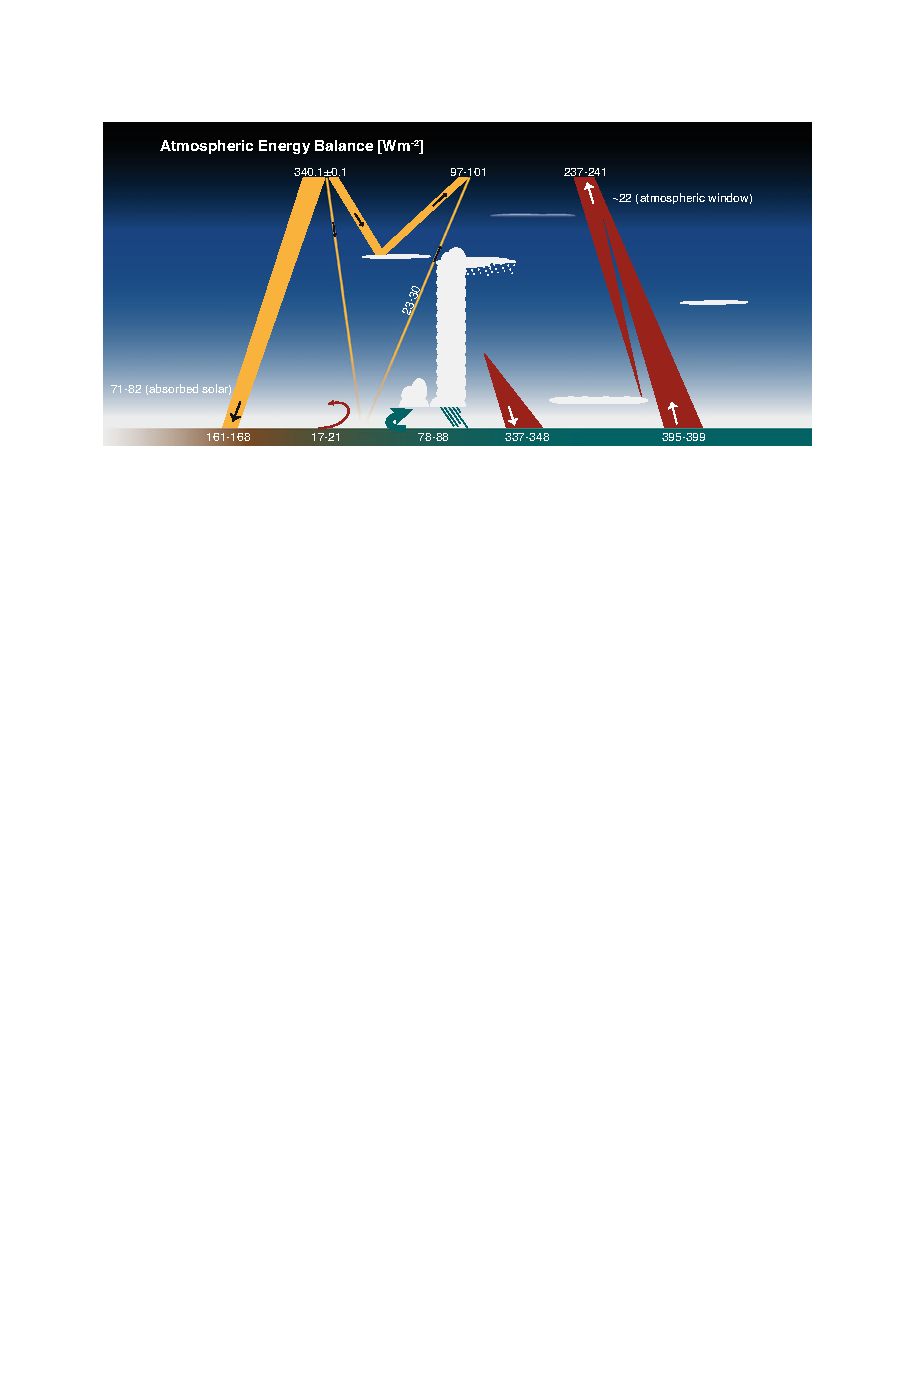
\includegraphics[width=15 cm]{../external_figures/Stevens_Schwartz_2012_energy_flows.pdf}
\end{center}
\caption{ Observational estimates of the Earth's energy balance from Stevens and Schwartz \citep{Stevens2012}. Yellow is sunlight, red is infrared radiation. The little whirl is turbulent sensible heat transfer and the green is latent heat transfer. } 
\label{fig:energy_flows}
\end{figure}

It is useful to consider the components of the global mean energy balance (Figure \ref{fig:energy_flows}). Here we consider the fluxes per meter squared surface area of the Earth (total area $510\cdot 10^{12}$ m$^2$). Energy flows in from the sun at 340 Wm$^{-2}$, about 100 of which are reflected back to space by clouds, aerosol particles or the surface. In the atmosphere some of the sunlight is absorbed, mostly by oxygen, ozone and water vapor, and the rest reaches and heats the surface. The surface gets rid of the heat again through emitting infrared radiation, and sensible and latent heat fluxes to the atmosphere. Of the emitted nearly 400 Wm$^{-2}$ infrared radiation most it is absorbed by the atmosphere

\begin{figure}
\begin{center}
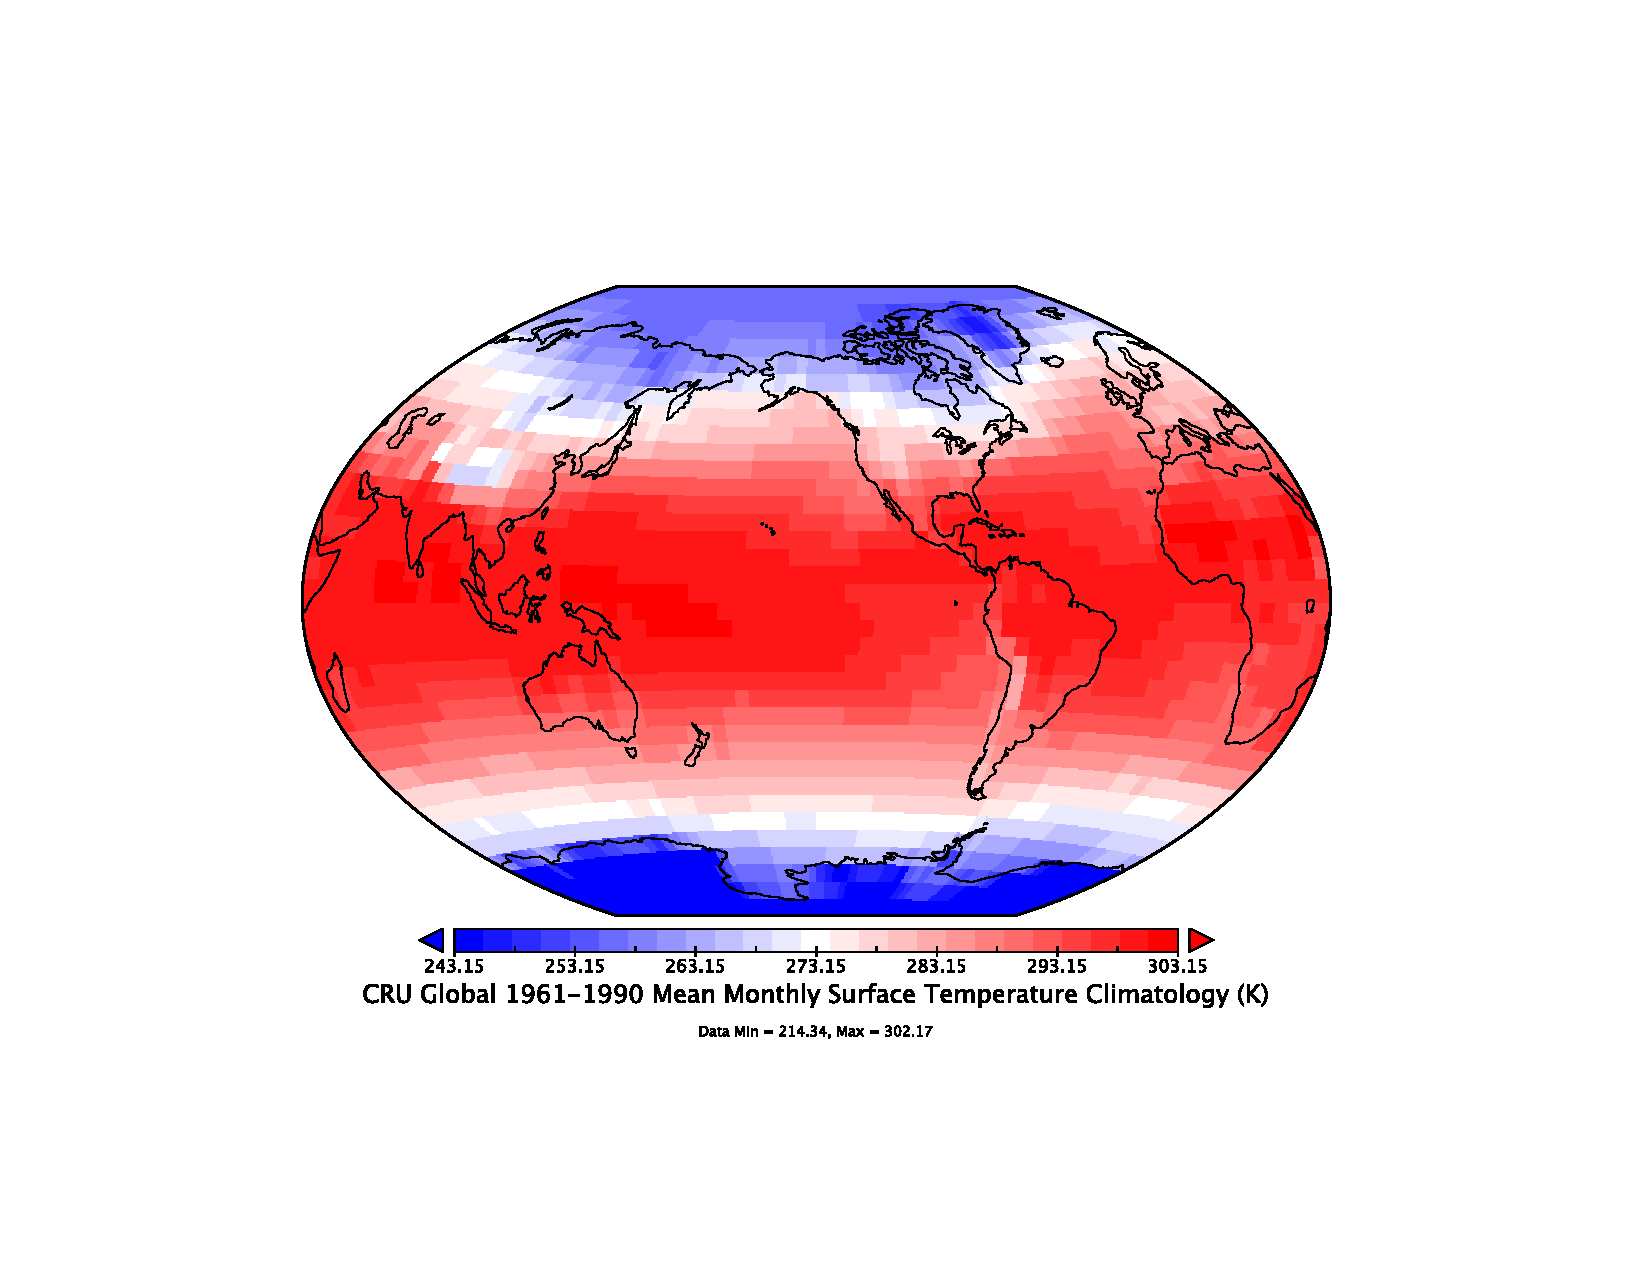
\includegraphics[width=12 cm]{../external_figures/HadCRUT_absolute_timmean.pdf}
\end{center}
\caption{ Observed annual mean near-surface temperature from HadCRUT. } 
\label{fig:HadCRUT_temperature_map}
\end{figure}

Partly because the sunlight is not distributed evenly over the Earth's surface it exhibits wildly varying temperatures near the surface with extremes from about -90$^\circ$C to +60$^\circ$C. Even in the annual longterm mean the coldest and warmest places differ by nearly 90 degrees (Figure \ref{fig:HadCRUT_temperature_map}). We will, however, often use a global mean surface temperature; today this is about 15$^\circ$C, or 288 K. These temperature gradients set up large energy flows in the atmosphere and oceans from warmer to colder regions. To get an idea of the magnitude of these transports one can inspect the zonal mean top-of-atmosphere radiation balance (Figure \ref{fig:ceres_fluxes}). The regions from about 36S to 36N receives more energy than is emitted back to space, whereas the high latitudes have an energy deficit. To compensate this, there must be a meridional energy transport from low to high latitudes in the oceans and in the atmosphere (It is left as an exercise to estimate the flux of energy from low to high latitudes). As a result, the temperature gradients on Earth are, in fact, modest. For instance, the Moon has equatorial temperatures varying from about 100 to 390 K between day and night, and even colder temperatures have been measured in craters near the poles.

\begin{figure}
\begin{center}
\includegraphics[width=12 cm]{../plots/CERES_Ebaf_zonalmean.pdf}
%\includegraphics[width=8 cm]{../plots/CERES_Ebaf_albedo.pdf}
\end{center}
\caption{ Top-of-atmosphere net fluxes of shortwave and longwave radiation as measured from satellite. The red area shows regions where more energy is received than emitted, it extends approximately from 36S to 36N and has a mean of 36.5 Wm$^{-2}$. The blue areas are regions that emit more radiation to space than they receive. In the Southern Hemisphere the mean flux is -54.0 Wm$^{-2}$ and in the Northern Hemisphere the deficit is -54.7 Wm$^{-2}$. Note that the x-axis is plotted as sinus of latitude such that the area under the curves can be integrated. } 
\label{fig:ceres_fluxes}
\end{figure}

On average, the coldest point in the Earth's troposphere is the tropical tropopause region with temperatures around 200 K (Figure \ref{fig:tropical_profiles}). These low temperatures are achieved through vertical mixing in deep convective clouds wherein localized rapidly rising motion causes adiabatic cooling due to the decreasing pressure with height. If the air was dry the temperature would decrease at a rate of about -10 K km$^{-1}$, but because some latent heat is released as water vapor condenses during the ascent, the actual lapse rate is less, about -6 K km$^{-1}$, tending towards the dry adiabat in the upper troposphere (Figure \ref{fig:tropical_profiles}). This is referred to as the moist adiabat.

Unlike the horizontal temperature gradients at the Earth's surface, mostly from equator to poles, that cause energy to be transported in the oceans and the atmosphere, the vertical temperature gradient of about 100 K in the topical troposphere is not on it's own causing transports to occur. However, as we shall see in a moment radiative cooling causes an upward convective  transport of energy to balance the budget of the atmosphere.

\begin{figure}
\begin{center}
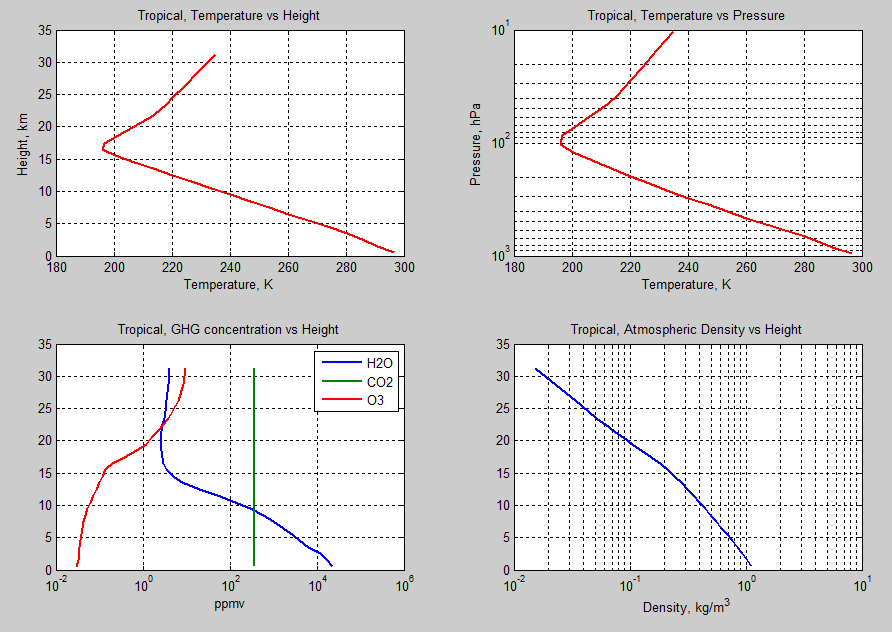
\includegraphics[width=17 cm]{../external_figures/atmospheric-radiation-13a-tropical-profile-temperature-gases-density}
\end{center}
\caption{ Typical tropical profiles of temperature as functions of height and pressure (top panels), volume mixing ratios of some greenhouse gases (lower left), and atmospheric density.  } 
\label{fig:tropical_profiles}
\end{figure}

\section{Radiative properties}
Let us next focus our attention on the infrared or longwave part of the Earth's radiation budget. A wealth of information can be obtained from studying the spectrum of radiation emitted from the Earth, stars and from other planets. This is because molecules have unique absorption properties that are determined by quantum mechanics. There are a number of ways in which atoms and molecules can absorb a photon, most of which happen at nearly discrete energies. Visible light is able to excite the electron states of atoms and highly energetic ultraviolet photons can split molecules apart. In the infrared, where photons each contain less energy, absorption happens mostly by exciting various modes of vibrations of molecules. 

Some molecules are unable to interact with infrared radiation, in fact the abundant nitrogen (N$_2$) and oxygen (O$_2$) molecules that constitute 99 percent of Earth's atmosphere are unable to absorb the low-energy infrared photons emitted by the Earth's surface. The simple configuration of these molecules with two atoms connected by electron bonds do not allow the absorption of a photon by vibration. More complex molecules with three or more atoms, such as water vapor (H$_2$O), carbon dioxide (CO$_2$), methane (CH$_4$) and ozone (O$_3$), can typically vibrate or rotate in a number of ways and are therefore what we call greenhouse gases. 

A useful starting point to appreciate the information in the infrared spectrum is to consider the radiation emitted by an ideal black body which constitutes a continuous and smooth spectrum called the Planck spectrum. Ideal black bodies are not necessarily black: if warm enough they can emit visible light, instead the blackness refers to them absorbing all incoming radiation perfectly, which is necessary to obtain the ideal emission spectrum because emissivity equals absorptivity. Examples of nearly ideal black bodies are the Sun, most solids and liquids. The surface of the Earth, be it the ocean or the land, is closely approximated as a black body. A cloud is also a surprisingly good absorber: a typical low-level liquid cloud consisting of suspended tiny droplets can be a nearly ideal black body if it contains a meager 20 gm${-2}$ of water. Gases, on the other contrary, are usually far from ideal black bodies. 

\begin{figure}
\begin{center}
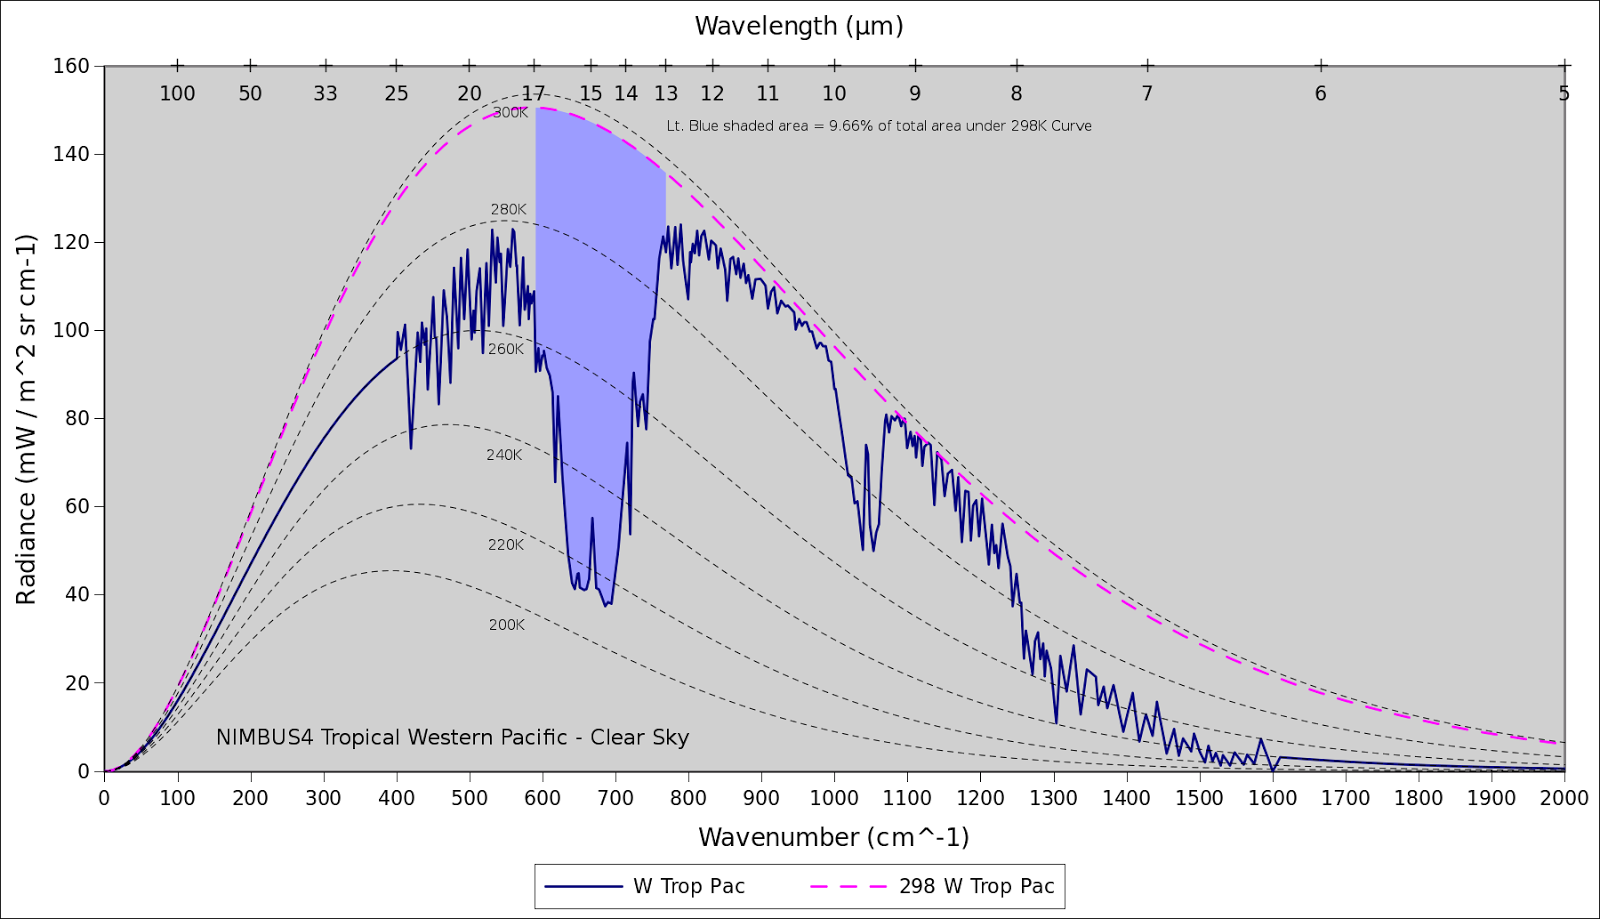
\includegraphics[width=17 cm]{../external_figures/GW_Petty_IRIS_Tropical_Western_Pacific.png}
\end{center}
\caption{ Classical irradiance spectrum measured by the infrared interferometer spectrometer (IRIS) for measuring the emission spectra of the earth/atmosphere system aboard the Nimbus-4 satellite. The instrument is limited to the range 400 to 1600 cm$^{-1}$, and outside simplistic extrapolations are made. The measurements were made in the 1970's and are restricted to clear sky scenes. Dashed lines show idealized black body spectra. Blue shading illustrates the effect of carbon dioxide (CO$_2$). The other dip at 1000-1100 cm$^{-1}$ is due to ozone (O$_3$), and the flanks (less than 600 and more than 1200 cm$^{-1}$) are dominated by vapor vapor (H$_2$O), as well as methane (CH$_4$) at around 1200-1400 cm$^{-1}$. In the atmospheric window between 10 and 13 $\mu$m there are multiple weak absorption lines from water vapor. } 
\label{fig:radiation_spectrum}
\end{figure}

Several spectra of such ideal black bodies are plotted in Figure \ref{fig:radiation_spectrum} for temperatures from 200 to 300 K as dashed lines. Also shown is the emission spectrum from a tropical cloud free scene as measured from space. The plot is linear in wavenumber such that shorter wavelength, corresponding to more energetic photons, are situated to the right. The warmer the black body the further both the peak and the tail extends to the right. For reference light that is visible to the eye is at 0.7-0.4 $\mu$m. Also the area under the spectra, which are proportional to the total irradiance from the black body which is a strong function of temperature:
\begin{equation}
R_b = -\sigma T^4,
\label{eq:blackbody}
\end{equation}
\noindent where $\sigma=5.67\cdot 10^{-8}$ Wm$^{-2}$K$^{-4}$ is the Stefan-Boltzmann constant. Most solids and liquids can be considered nearly ideal black bodies, including the Earth's surface. Also thick clouds act as if they were nearly ideal black bodies.

Now, let us compare the ideal black body spectra with the actual spectrum measured over the tropical Pacific (Figure \ref{fig:radiation_spectrum}): The observed spectrum is indeed far from ideal, which is a consequence of the atmosphere being between the satellite and the Earth's surface. Parts of the spectrum (10-13 $\mu$m), sometimes referred to as the atmospheric window, are actually quite close to the black body spectrum of the surface temperature in this tropical region (298 K), but other parts are much colder, 215 K at about 15 $\mu$m, or considerably colder with 260-270 K at both long and short wavelengths. We call these brightness temperatures as they are the equivalent irradiance of an ideal black body.
The reason that parts of the spectrum is suppressed relative to that of a black body with the surface temperature is that it is not only the surface that is emitting but also the greenhouse gases of the atmosphere absorb and emit radiation. The temperature with which they effectively emit is a result of the individual molecules absorption properties, their mixing ratio profiles, and the atmospheric density and temperature profiles (Figure \ref{fig:tropical_profiles}):
\begin{itemize}
\item
Take first carbon dioxide (CO$_2$). It has a uniform and relatively high mixing ratio and it absorbs well around 13-17 $\mu$m (Figure \ref{fig:radiation_spectrum}, blue shading). The result is that most of the emission in the band around 15 $\mu$m comes from the upper troposphere where the atmospheric density is still high enough. Above the tropopause (about 18 km) the temperature rises again, and actually some of the emission in the center of the CO$_2$ dominated band originates in the stratosphere which is somewhat warmer than the troposphere as marked by a spike. 
\item
For the water vapor (H$_2$O) dominated flanks of the spectrum, however, the story is different. Water vapor is most abundant in the lower troposphere (Figure \ref{fig:tropical_profiles}), and most of the radiation emitted by water vapor originates from there. This results in the Earth's spectrum being closer to that of a black body with 260-270 K at the flanks consistent with temperatures at about 5-7 km in the tropics.
\item
Finally, let us consider ozone (O$_3$) which increases in mixing ratio with height and is most abundant in the stratosphere where it is produced by photodissociation of oxygen molecules by an ultraviolet photon ($\nu$): 2O$_2 +\nu$ $\rightarrow$ 2O + O$_2$ $\rightarrow$ O + O$_3$ $\rightarrow$ 2O$_2$. Most of the ozone mass is at 20-25 km altitude, whereas the volume mixing ratio peaks higher up at 30-40 km. Ozone absorbs infrared radiation at 9-10 $\mu$m wavelength where we see a brightness temperature of about 270-280 K. Most of this radiation originates in the stratosphere, which is warmer than the upper troposphere, and therefore the depression is not as deep as for the CO$_2$ case.
\end{itemize}
I hope you have now a bit of an impression of the power of the infrared spectrum. We shall return to it on later occasions. 

\section{The tropopause}
The transition zone between the troposphere and the stratosphere plays a central role in several of the themes related to the dynamics of climate. The tropopause plays a key role in determining the forcing from greenhouse gases, and it is central to understanding certain feedback mechanisms.

Perhaps a good starting point is the now iconic single-column simulations by Manabe and Strickler presented in their 1964-paper\citep{Manabe1964} (Figure \ref{fig:rce_manabe}). In their model they prescribed profiles of ozone and water vapor, and let the sun shine. A large fraction of the sunlight passes to the surface which is relatively warm. In the simplest case of a pure radiative equilibrium the surface reaches about 340 K whereas the troposphere is colder than observed. The pure radiative equilibrium is that the radiation absorbed and emitted at a given level is equal. However, in case the temperature drops this quickly with height then convective instability will occur. To parameterize this Manabe and Strickler adjusted the profile to first a dry adiabat (-10 K/km) and then to a more realistic lapse-rate close to the moist adiabat (-6.5 K/km). The result is that the troposphere is warmer and the surface is colder than at pure radiative equilibrium. Note how the stratosphere is not reacting much. Here instead the temperature rises with altitude and therefore no convective instability arises. The stratosphere also cools in the infrared, but it is being heated by absorption of sunlight mostly by the ozone layer. In summary: the convection acts to heat the troposphere in order to compensate radiative cooling -- we say it is in radiative-convective equilibrium (RCE) -- whereas the stratosphere is roughly in a radiative equilibrium. 

\begin{figure}
\begin{center}
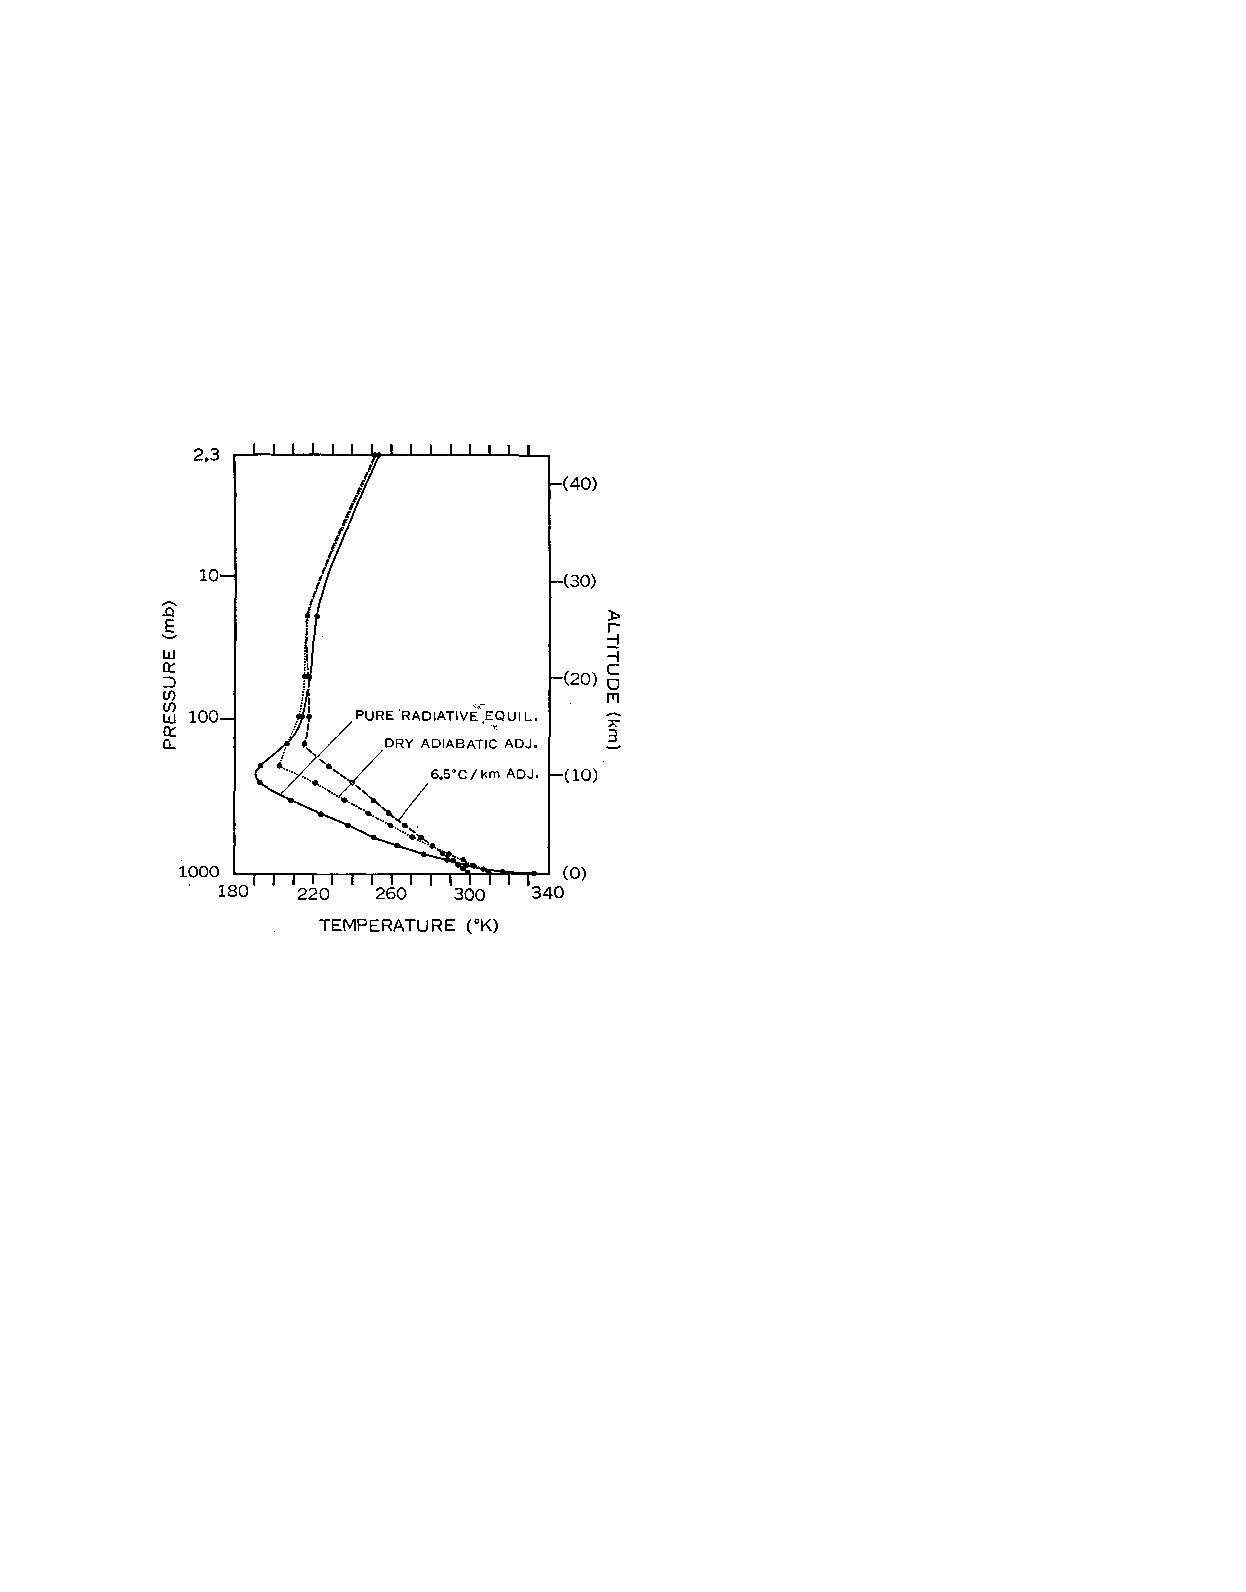
\includegraphics[width=10 cm]{../external_figures/Manabe_Strickler_1964_figure.pdf}
\end{center}
\caption{ Solutions to radiative and radiative-convective equilibrium in the single-column model by Manabe and Strickler\citep{Manabe1964}.   } 
\label{fig:rce_manabe}
\end{figure}

It is the greenhouse gases that act to cool the troposphere by emitting infrared radiation through radiative flux divergence. If we define a net flux as the difference between an upward and a downward component ($R_{net}(z) = R^\downarrow(z) - R^\uparrow(z)$, where $z$ is height), then we can calculate the heating rate as:
\begin{equation}
\frac{dT}{dt} = \frac{1}{c_p \rho}\frac{dR_{net}}{dz},
\end{equation}
where $c_p$ is the heat capacity of air and $\rho$ the density of air. Figure \ref{fig:radiative_cooling} shows infrared heating rates that are due to individual greenhouse gases in the tropical cloud-free profile displayed in Figure \ref{fig:tropical_profiles}. The heating rates are mostly negative and on the order of degrees per day, that is, if no other process would be acting to keep the temperature in place it would change at this rate. Ozone is the exception which heats the atmosphere in the lower stratosphere. But above 30 km ozone is also cooling the atmosphere, and it does so by radiating both upwards and downwards. It is partly this downwards flux from the warm upper stratosphere aloft that is being absorbed in the colder lower stratosphere. There are at least three controls that conspire to have the troposphere where it is:
\begin{itemize}
\item
Water vapor dominates infrared cooling in the troposphere, and is the reason that the pure radiative equilibrium case of Manabe and Strickler (Figure \ref{fig:rce_manabe}) has such a cold troposphere. However, water vapor mixing ratio decreases rapidly with height because the holding capacity decreases with temperature according to Clausius-Clapeyron. At around 15 km altitude, or more importantly around 200 K temperature, the cooling due to water vapor is nearly zero. It is thought that in a warming climate the tropical tropospheric temperature will increase to maintain roughly a moist adiabat, such that the level at which the temperature reaches 200 K moves upward, and with it the water vapor cooling and consequently the tropopause (Hartmann and Larsson\cite{Hartmann2002}). {\em Radiative cooling by water vapor comes to an end.}
\item
Another way to look at this is that the heating caused by moist convection, which is to compensate the radiative cooling, can only function as long as the moist and dry adiabats are different. The ascending air inside deep convective clouds follow approximately the moist adiabat which generally has a lower lapse-rate of temperature with height than the dry adiabat. The heating due to convection occurs as the surrounding air subsides, as a result of continuity, instead along a dry adiabat. However, at very cold temperatures, around 200 K, the moist and dry adiabats are practically the same as there is very little water vapor left to condense, and it follows that the convection can no longer heat the troposphere. This sets another control on the tropopause height. {\em Heating by moist convection comes to an end.}
\item
Absorption of sunlight by ozone is the main source of heating in the stratosphere and results in the increasing temperature with height which hinders convection from penetrating deeper. Ozone has a relatively long lifetime in the stratosphere but if it ends up in the troposphere it is quickly destroyed. So the ozone layer has to move up to stay above a rising tropopause in a warming climate. If this leads to a thinning of the ozone layer perhaps more ultraviolet radiation can penetrate into and heat the upper troposphere, thereby increasing the temperature of the tropopause. {\em Ozone heating may bound the rise.}
\end{itemize}
Understanding the actual behavior of the tropopause is a field of active research, and the rise of the tropopause with warming plays an important role in determining climate change feedbacks. 

\begin{figure}
\begin{center}
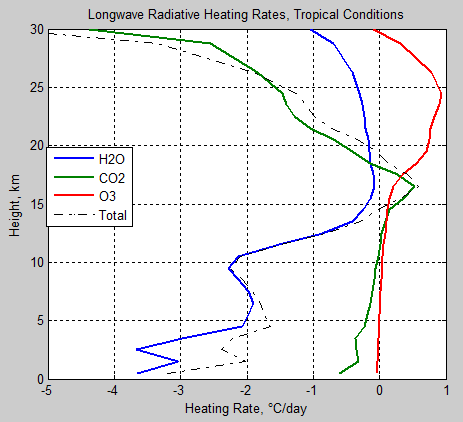
\includegraphics[width=8 cm]{../external_figures/atmospheric-radiation-13c-heating-rates-tropical-each-h2o-co2-o3.png}
\end{center}
\caption{ Longwave heating rates due to individual greenhouse gases calculated for the  clear-sky tropical atmosphere displayed in Figure \ref{fig:tropical_profiles}.  } 
\label{fig:radiative_cooling}
\end{figure}


%\section{Energy transports}
%The atmosphere and oceans transport energy

\newpage
\vspace{2 cm}
%\hrule
{\setlength{\parindent}{0cm}
\begin{exercise}
Estimate the combined poleward energy transport by the atmosphere and oceans at 36N based on Figure \ref{fig:ceres_fluxes}. Do this by estimating the area poleward of that latitude; the result should be given in PW.
\end{exercise}

\begin{exercise}
Estimate roughly from which heights in the troposphere thermal radiation to space comes from. Use Figures \ref{fig:tropical_profiles} and \ref{fig:radiation_spectrum} and divide into lower-, mid- and upper troposphere by means of its temperature. Use the fact that the area under the curve in Figure  \ref{fig:radiation_spectrum} is the total flux. %Next, compare the amount of radiation escaping to space at near-surface brightness temperature to the amount escaping through the atmospheric window in Figure \ref{fig:energy_flows}. What is the difference do you think? 
\end{exercise}

\begin{exercise}
Explain, in your own words, why the tropopause is where it is.
\end{exercise}

\begin{exercise}
Visit the MODTRAN infrared radiation model at http://climatemodels.uchicago.edu/modtran/. This is a graphical interface to a moderately resolved radiative transfer model. By default the model uses a tropical cloud-free profile with present-day greenhouse gases, and the spectrum is what one might observe looking down from 70 km altitude, i.e. at the top of the stratosphere. You can always revert to these settings by reloading the webpage. Starting from these settings, hit the {\em Save this run to background} button. The saved run will later appear as a red line. Now place yourself at the tropopause. What is the difference?
\end{exercise}
}

% TASKS:
%
% Make sure you have python access, including numpy and matplotlib (preferably Anaconda)
%
% Assume the Earth's surface is a black body and calculate it's temperature based on the emission in Figure \ref{fig:energy_flows}. Assume it is 1 K warmer, then how much more does it radiate? How much of this flux will approximately escape directly to space through the atmospheric window?
%
% Estimate from which heights in the troposphere thermal radiation to space comes from
% Estimate the fixed anvil temperature (FAT) cloud feedback by assuming a fixed areal coverage of anvils and a fixed tropospheric lapse-rate
%
% Show that the short term response to an abrupt forcing does not depend on lambda.
%
% Show that T(t) is a solution to the two-layer model to an abruptly applied forcing, draw the two components of the solution as a function of time and their sum 
% 
% Assume a polynomial behavior of lambda, estimate max and minimum ECS
% Estimate steric sea-level rise in two-layer model
% Assume X percent of the top-of-atmosphere energy imbalance goes to 
%
% Does FAT depend on the temperature of the surface?

% Imagine one alternative cause of historical warming (e.g. solar forcing, ozone depletion, geothermal heating, galactic particles). How would you go about testing this hypothesis?

%---------------------------------------------------------------------
\chapter{Energy balance}
The flows of energy in and out of the planet is central to climate dynamics; it is actually more important to keep track of the energy balance than it is to trace surface temperature which  represents only a small part of the Earth's total heat reservoir. The temperature, however, plays a central role in determining this balance: in essence a planet receives energy at some rate and therefore warms up until it loses energy at the same rate. In fact, whereas a planet in general can receive energy in a number of ways, infrared radiation is basically the only way in which it can get rid of it again.

\section{The black body case}
Most of the Earth's energy is received from the Sun in the form of shortwave radiation, sunlight. At the Earth's distance from the Sun this corresponds to a flux of little more than 1360 Wm$^{-2}$ through a sphere centered at the Sun. This number is often referred to as the solar constant, or $S_o$, although it is not really to be considered constant. There are other small sources of energy such as geothermal heat from the interior of the Earth and heat generated by dissipation of tides, but these can be safely neglected. On other planets or moons, however, this need not be the case.

Because the distance between the Sun and the Earth is vast compared to their respective radii, we can assume that all incoming sunlight is parallel, which makes it easy to calculate the average sunlight per unit area of the Earth's surface. The radiation is intercepted by the Earth cross-section which is roughly that of a disc with the average radius of the Earth ($r$), or $\pi r^2$. But the surface area of the Earth is larger, roughly $4\pi r^2$. It follows that the intercepted sunlight must be spread over a four times larger area, giving a mean incident flux of about 340 Wm$^{-2}$. In addition, not all the incoming sunlight is absorbed, but as we saw in the previous chapter about 100 Wm$^{-2}$ is reflected back to space by clouds, aerosol particles and the surface. We say that the Earth has a planetary albedo of $\alpha \approx 100/340 \approx 0.29$. It follows that the absorbed sunlight is $R_s=(1-\alpha)S_o/4$. Finally, we shall assume that the Earth's surface has a single uniform temperature, that it radiates to space as an ideal black body following Equation \ref{eq:blackbody}, and that the atmosphere is fully transparent to infrared radiation.
Now we are in a position to form a first estimate of the energy balance ($N$) :
\begin{eqnarray}
N &=& R_s + R_b \nonumber \\ 
   &=& \frac{S_o}{4}(1-\alpha) - \sigma T_e^4,
\label{eq:black_body_energy_balance}
\end{eqnarray}
\noindent where $T_e$ is an effective, or emission, temperature of the Earth that it would have had had it been an ideal black body. The balance  can be solved by setting $N=0$:
\begin{equation}
T_e = \sqrt[4]{S_o(1-\alpha)/4\sigma}. 
\end{equation}
Inserting reasonable values we obtain $T_e \approx$  255 K. This is considerably colder than the global mean surface temperature of the Earth ($T_s$) which is currently about 288 K. But remembering the observed spectrum of Earth in Figure \ref{fig:radiation_spectrum} perhaps this is not too surprising; a large part of the spectrum is at a lower brightness temperature than that of the surface. The found emission temperature is that of the ideal black body that would average the Earth's infrared radiance to space (remember the observation in Figure \ref{fig:radiation_spectrum} is a cloud-free scene from the tropics which is warmer than average).

\section{The greenhouse effect}
The reason the surface of the Earth is about 33 K warmer than the emission temperature is the so-called greenhouse effect, which was first suggested to exist by Fourier in his essay from 1827; a nice 1-page perspective on that paper is provided by Pierrehumbert \cite{Pierrehumbert2004}. Fourier formulated the question of what determines Earth's temperature and developed the idea of the planetary energy balance which is the foundation of climate science. 

\begin{figure}
\begin{center}
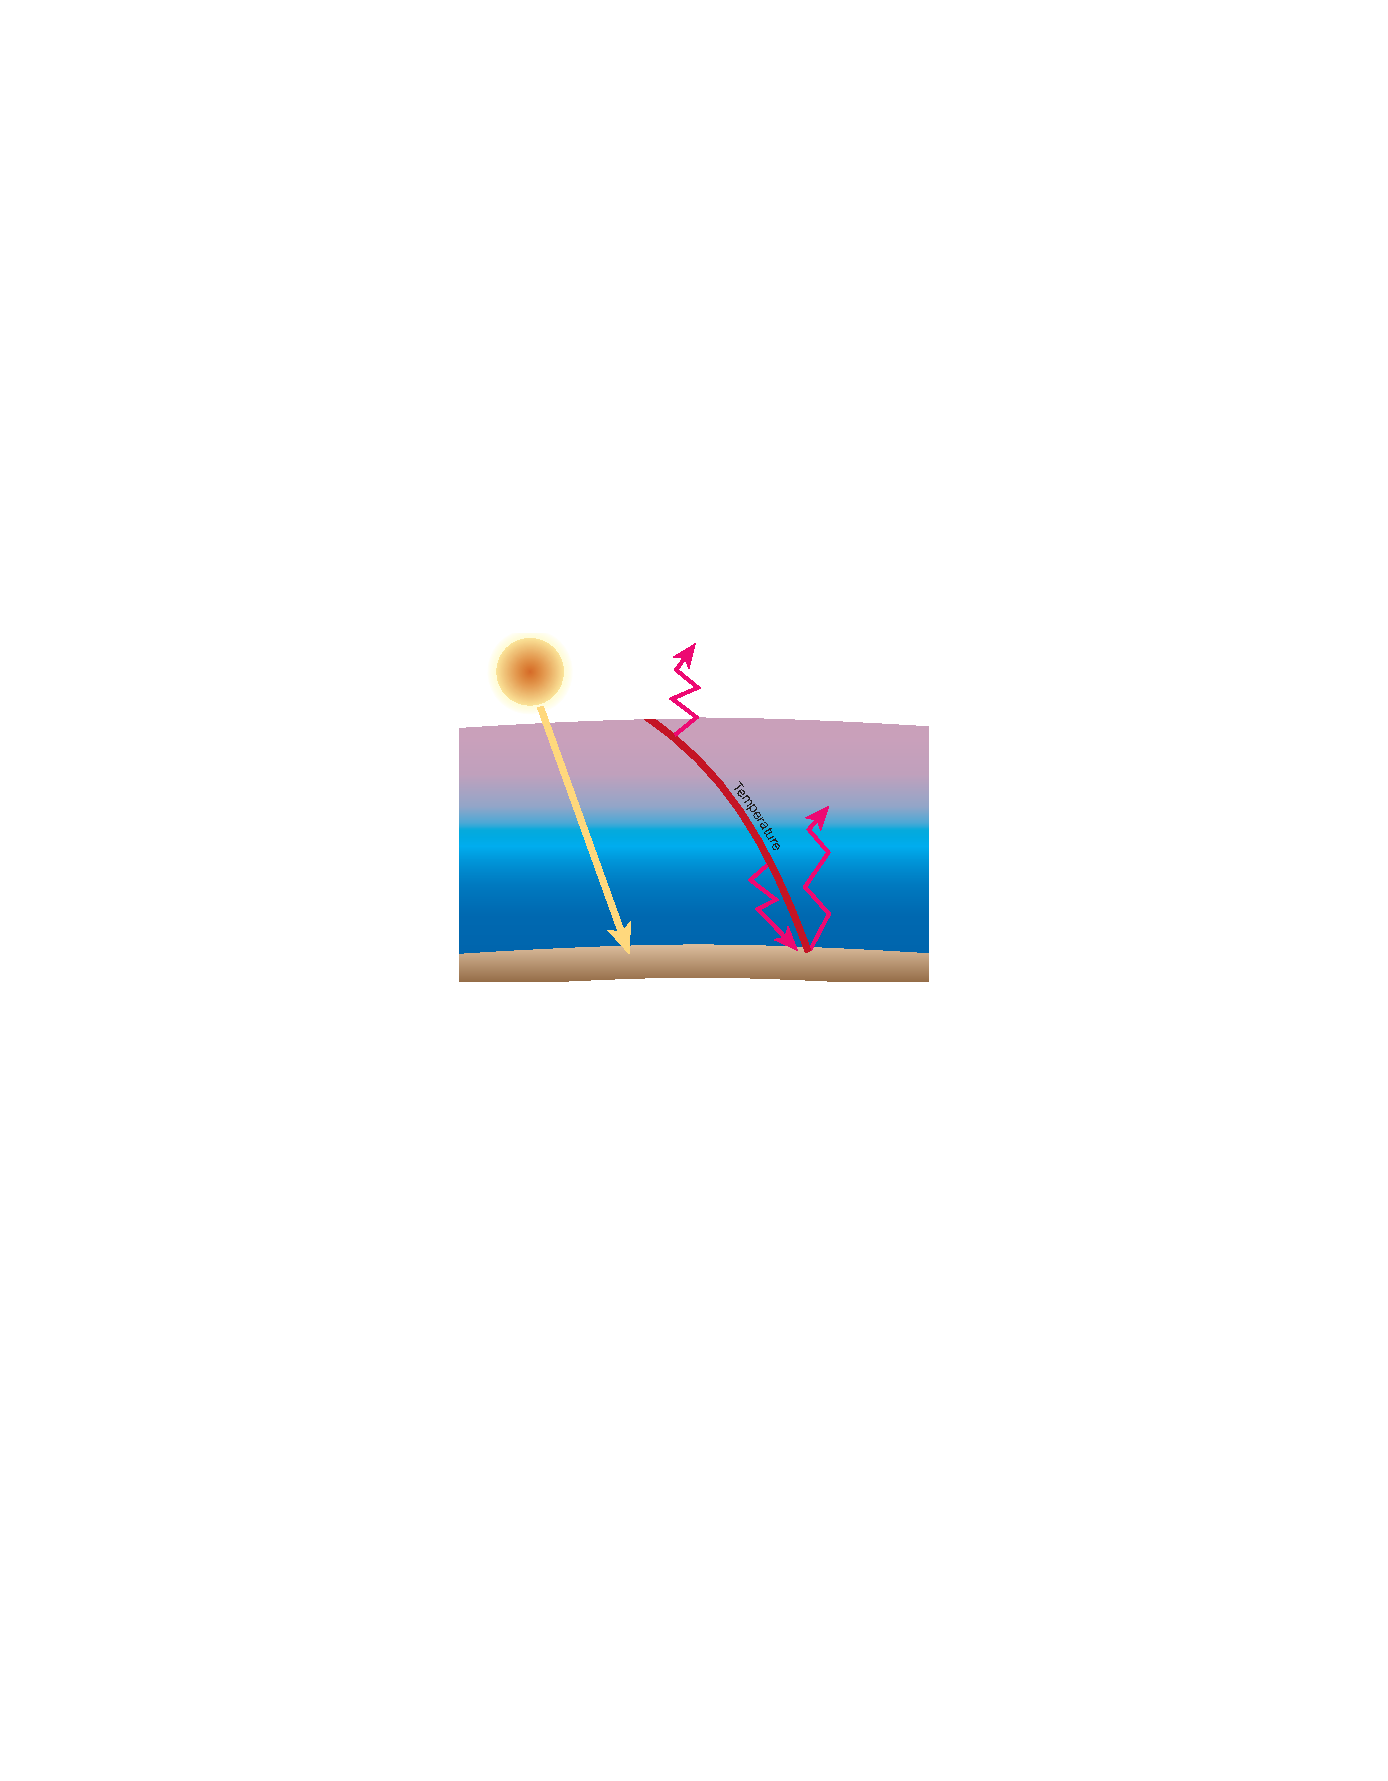
\includegraphics[width=8 cm]{../external_figures/Greenhouse_effect_illustration_Pierrehumbert_2004}
\end{center}
\caption{ Illustration of the greenhouse effect by Pierrehumbert \cite{Pierrehumbert2004}. Heat is lost by infrared radiation (pink arrows) but some of that emitted by the warm surface is absorbed and re-emitted by the cooler troposphere. The thick red line shows an idealized temperature profile. The result is that the surface has to become warmer compared to the case when there is no atmosphere in order to obtain energy balance.    } 
\label{fig:greenhouse_effect_illustration}
\end{figure}

It is often argued that the naming of the greenhouse effect is misleading. The greenhouses, which we use to grow vegetables and fruits, are indeed warmer than their surroundings because sunlight is trapped inside, but they are warmer mainly because they hinder air motion from transporting the excess heat away. This is fundamentally different from how the atmospheric greenhouse effect works which is by absorbing infrared radiation emitted by the surface and re-emitting at a lower temperature to space resulting in a warmer surface (Figure \ref{fig:greenhouse_effect_illustration}). We can define the greenhouse effect as the difference between the infrared radiation emitted by the surface ($R^\uparrow_{ir}(\textrm{sfc})$) and that which escapes to space ($R_{ir}(\textrm{toa})$), and then assume the fluxes are consistent with those of black bodies at the emission- and surface temperatures:
\begin{eqnarray}
\textrm{Greenhouse effect}&\equiv&   R_{ir}(\textrm{toa}) - R^\uparrow_{ir}(\textrm{sfc}) \nonumber \\ 
                                           &\approx&   -\sigma (T_e^4 - T_s^4) \nonumber \\
                                           &\approx& 150 \ \textrm{Wm}^{-2}, \nonumber
\end{eqnarray}
which is a bit less than the estimate by Stevens and Schwartz of 155-160 Wm$^{-2}$ (Figure \ref{fig:energy_flows}). It is easy to understand why our estimate is smaller. The black body radiation depends on the temperature to the fourth power and so if there are inhomogeneous distributed surface temperatures, such as is the case at Earth's surface ($T_s$), then the average emitted radiation is larger than that of a uniform black body with the same average temperature.

\section{The perfectly absorbing slab atmosphere}
To emulate a greenhouse effect we may consider a single-temperature, or slab, atmosphere that is perfectly transmissive to sunlight but a black body absorber in the infrared. We may think of this as a slab of perfect greenhouse gas. The atmosphere radiates up and down as an ideal black body. At the top of this atmosphere (toa) the same energy balance must hold as for the pure black body case (Eq. \ref{eq:black_body_energy_balance}). At the surface (sfc), in addition to the unhindered downwelling solar irradiance, also downwelling infrared radiation comes from the atmosphere, while the surface radiates upward: 
\begin{eqnarray}
N_\textrm{toa} &=&  \frac{S_o}{4}(1-\alpha) - \sigma T_e^4  \\ 
N_\textrm{sfc} &=&  \frac{S_o}{4}(1-\alpha) + \sigma T_e^4 - \sigma T_s^4  \nonumber
\label{eq:perfect_greenhouse}
\end{eqnarray}
and at equilibrium we have energy balances both at the top-of-atmosphere and at the surface, $N_\textrm{toa}=N_\textrm{sfc}=0$, so that we can solve for surface temperature for a single layer atmosphere:
\begin{equation}
T_s(1) = \sqrt[4]{S_o(1-\alpha)2/4\sigma}. 
\end{equation}
Putting in reasonable numbers we obtain a surface temperature of 304 K -- substantially warmer than that on Earth -- and a whopping greenhouse effect of 243 Wm$^{-2}$. Now, let us double the amount of our perfect greenhouse slab by adding another layer to obtain the solution (it is left as an exercise to show this):
\begin{equation}
T_s(2) = \sqrt[4]{S_o(1-\alpha)3/4\sigma},
\label{eq:ntwo}
\end{equation}
or in the general case with $n$ levels:
\begin{equation}
T_s(n) = \sqrt[4]{S_o(1-\alpha)(n+1)/4\sigma},
\end{equation}
such that the temperature increases monotonically with the number of perfect greenhouse slabs. Eventually, the approximations made above must break down when the surface gets so hot that it radiates visible light which can escape unhindered through this idealized atmosphere. 

Obviously, and perhaps luckily, we do not have such a perfect greenhouse slab in the Earth's atmosphere, rather individual gases only absorb in parts of the infrared spectrum. In the bands around 15 $\mu$m where CO$_2$ absorbs the atmosphere is virtually opaque to radiation, but at other wavelengths infrared radiation from the surface or lower troposphere can escape to space (Figure \ref{fig:radiation_spectrum}). It is sometimes incorrectly argued that because the atmosphere is nearly saturated in the CO$_2$ absorption bands then adding more will not act to warm the Earth's surface. However, the example above with $n$ completely opaque greenhouse gas slabs nicely illustrates the opposite: the more slabs you add, the warmer is your surface temperature.

\section{The partially absorbing slab atmosphere}
It is therefore useful to think of the atmosphere as partially absorbing. Commonly this is modelled using an effective emissivity that is less than unity, sometimes referred to as the gray body case, or gray radiation case. 
It is the purpose of an exercise to study this case and estimate the effective emissivity of the Earth and to show that the result is analogous to what we shall find below. 
Perhaps a physically more revealing approach is to consider an atmosphere layer analog to the perfect greenhouse case above that transmits all solar radiation but absorbs and emits in only a fraction $f$ of the infrared spectrum. The problem is illustrated in Figure \ref{fig:partially_absorbing_atmosphere}.

\begin{figure}
\begin{center}
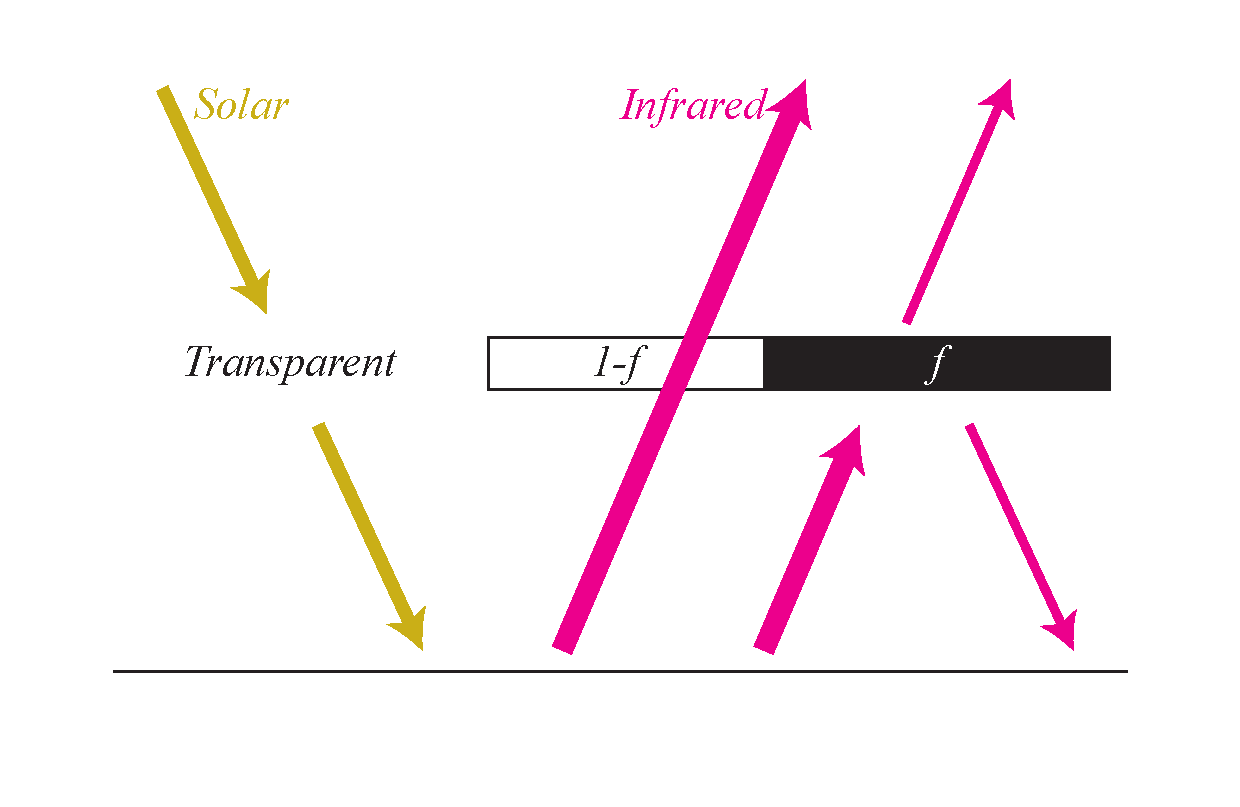
\includegraphics[width=12 cm]{../illustrations/Partially_absorbing_atmosphere}
\end{center}
\caption{ The energy balance for the partially absorbing slab atmosphere.    } 
\label{fig:partially_absorbing_atmosphere}
\end{figure}

Now, let $T_s$ be the surface temperature and $T_a$ be the atmosphere temperature. Unlike in the perfect greenhouse slab case, we cannot assume that the atmosphere temperature equals the emission temperature, $T_e$. We can then set up balances at the top of the atmosphere and at the surface:
\begin{eqnarray}
N_\textrm{toa} &=&  \frac{S_o}{4}(1-\alpha) - f \sigma T_a^4 - (1-f)\sigma T_s^4 \nonumber \\ 
N_\textrm{sfc} &=&  \frac{S_o}{4}(1-\alpha) + f \sigma T_a^4 - \sigma T_s^4 \nonumber 
\end{eqnarray}
Again, we can assume stationarity and solve for $T_s$ and $T_a$:
\begin{equation}
T_s(f) = \sqrt[4]{\frac{S_o(1-\alpha)}{2\sigma(2-f)}}, \ T_a(f) =  \sqrt[4]{\frac{S_o(1-\alpha)}{4\sigma(2-f)}},
\label{eq:partial_absorbtion_solution}
\end{equation}
such that we see that $T_s > T_a$ under all conditions and that they both increase with increasing $f$. For the limit $f \rightarrow 1$ we obtain $T_a \rightarrow T_e$ as in Equation \ref{eq:perfect_greenhouse}, and in the opposite case $f \rightarrow 0$ we obtain $T_s \rightarrow T_e$ as in the ideal black body case of Equation \ref{eq:black_body_energy_balance}. We may also solve for $f$ instead:
\begin{equation}
f = 2 - \frac{S_o(1-\alpha)}{2\sigma T_s^4},
\end{equation}
which for Earth-like conditions gives $f \approx 0.76$, that is, three quarters of the infrared radiation emitted from the surface has to be absorbed by the greenhouse slab if we are to get a surface temperature of 288 K. To obtain balance here, the atmosphere has to be colder than $T_e$, about 242 K. We can understand this as some of the radiation can escape from the surface directly space, so that to obtain energy balance with the incoming solar radiation the atmosphere has to be colder than 255 K such that the average emission temperature is $T_e$. In the limit $f \rightarrow 0$ the atmospheric temperature is about 215 K, but of course, strictly in the limit that temperature looses meaning as no radiation is absorbed and emitted from the atmosphere anymore.


\section{Greenhouse effect of a gaseous atmosphere}
Now in practical cases the atmosphere does not consist of a single, or multiple slabs in radiative equilibrium with the incoming solar radiation and the outgoing infrared radiation, rather it consists of gases, clouds and perhaps some particulate matter. An important property of a gaseous atmosphere is that it is relatively mobile, so that it can overturn and react on timescales comparable to those of radiative heating and cooling. As a first approximation we can think of this by the troposphere having a reasonably fixed lapse-rate with height. For dry mixing this would be about -10 K/km, but as discussed earlier the real atmosphere cools less rapidly with height due to release of latent heat in convective clouds.

\begin{figure}
\begin{center}
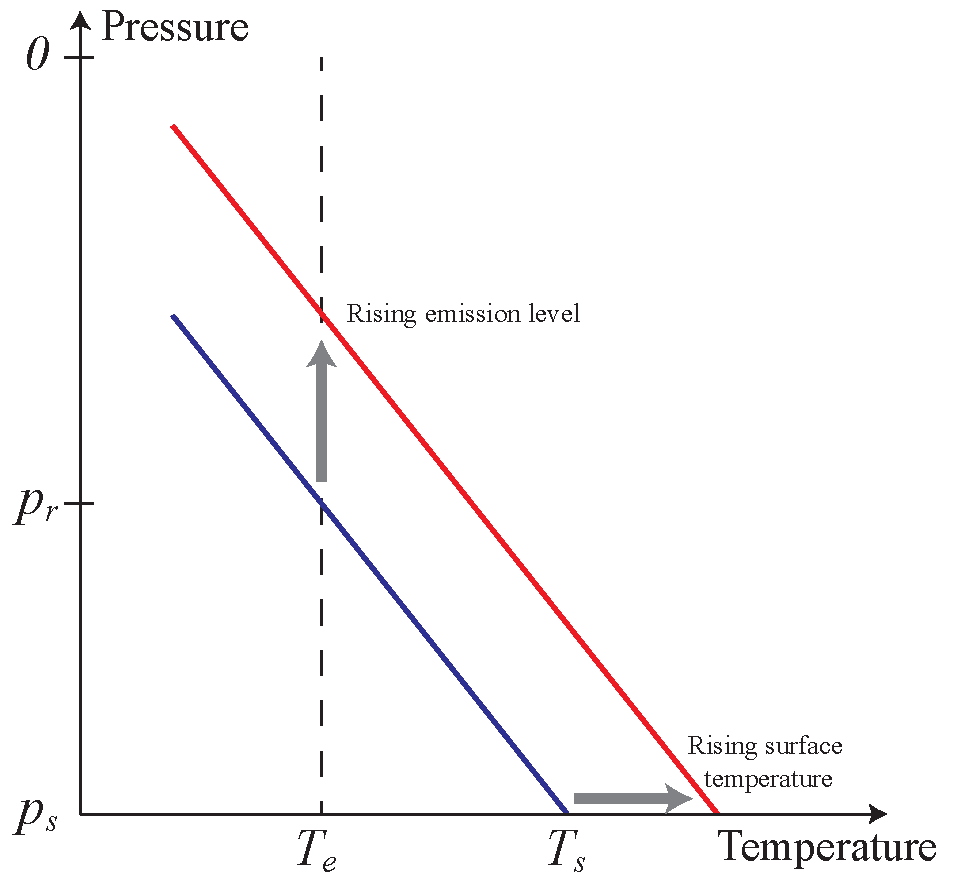
\includegraphics[width=8 cm]{../illustrations/Gaseous_atmosphere_radiation_level}
\end{center}
\caption{ Illustration of the concept of a radiation level pressure for an optically thick atmosphere. With more greenhouse gas (red) the radiation level moves upward and therefore the surface and atmosphere has to warm in order to again radiate as $-\sigma T_e$ to space.   } 
\label{fig:radiation_level}
\end{figure}

Let us start with an atmosphere that is fully transparent to infrared radiation. Here we may think of the Earth's dry atmosphere absent of carbon dioxide, ozone, methane etc. That is, it could for instance consist of nitrogen or oxygen. Then we are effectively having the black body case (Eq. \ref{eq:black_body_energy_balance}) wherein $T_s = T_e$. Then let us add some small amount of a perfect greenhouse gas, one that absorbs equally well at all infrared wavelengths. We shall assume that it is equally distributed everywhere, such as is the case for carbon dioxide (Figure \ref{fig:tropical_profiles}), with a concentration $q$. Trace gas concentrations are fractions typically measured in parts per million (ppm) or parts per billion (ppb).

As we look at this atmosphere from space the radiation emitted towards us is then  a mixture of radiation from different heights. If $q$ is very small some of the radiation emitted by the surface may escape directly to space without being absorbed by the greenhouse gas molecules: some of the photons can slip through, and we call the atmosphere optically thin. In the other limit, if $q$ is large then even a small fraction of the atmospheric column can act as if it was a black body. The pressure thickness of such a layer will scale with the amount greenhouse molecules, $q \Delta p/g$, such that the larger $q$ is, the smaller $\Delta p$ has to be. As we view our optically thick atmosphere from space we will almost exclusively see radiation coming from the uppermost part ($\Delta p$) and it will be characterized by the temperature that prevails in this layer. In this case it may be useful to think of the infrared radiation as coming from a certain radiation level, $p_r < p_s$, that is the height at which the temperature equals the emission temperature, $T_e$. The concept is illustrated in Figure \ref{fig:radiation_level}.

As we add more greenhouse gas to our atmosphere then the pressure thickness, $\Delta p$, required to act as a black body decreases, and so with it $p_r$ becomes smaller. Therefore the emission level moves upward in the atmosphere to lower pressure. But since the emission temperature, $T_e$, is constrained to be that which closes the energy budget of the planet (in the case of Earth $T_e \approx 255$ K) then the whole atmosphere as well as the surface has to warm up. This is because the surface and atmosphere are dynamically coupled by mixing processes to follow closely a certain lapse-rate.

In a nutshell, the reason there is a greenhouse effect is that the atmosphere absorbs some of the radiation emitted by the surface and re-emits at a lower temperature to space. To achieve this the atmosphere has to be colder than the surface; something which is ensured through convective mixing.


\section{A note on signs}
As you may have already noticed, throughout this set of notes I will count all fluxes as positive downwards. This has the advantage that positive fluxes will act to warm- and negative fluxes cool the system. Likewise, the feedback parameter that we shall define in the next chapter is automatically negative for stable climates and positive for unstable climates. The downside is that the {\em outgoing longwave radiation} emitted by the Earth (OLR) is then a negative flux -- where possible I shall denote it {\em net longwave radiation} trying to avoid confusion. Also note that some figures that I borrow can use the definition where OLR is positive. In the literature a number of sign conventions have developed, and it is worth paying close attention when reading on.

%\newpage
\vspace{1 cm}
{\setlength{\parindent}{0cm}
\hrule
\begin{exercise}
Show that the energy balance for the gray body case leads to this expression of the equilibrium surface temperature:
\begin{equation}
T_s = \sqrt[4]{\frac{S_o(1-\alpha)}{4\epsilon\sigma}}.
\label{eq:gray_radiation}
\end{equation}
Do this by modifying Equation \ref{eq:black_body_energy_balance} replacing $\sigma T_e^4$ with $\epsilon \sigma T_s^4$, where $\epsilon$ is the emissivity. Compare the result with the partially absorbing atmosphere, Equation \ref{eq:partial_absorbtion_solution}, and find out how $\epsilon$ depends on $f$. How small can $\epsilon$ be for a single slab atmosphere? And for $n$ slabs? Estimate the Earth's effective emissivity by solving Equation \ref{eq:gray_radiation} for $\epsilon$.
\end{exercise}

\begin{exercise}
Derive Equation \ref{eq:ntwo} for a two-layer atmosphere in the same way as done for the case for the single-layer atmosphere.
\end{exercise}

\begin{exercise}
Make sure you have access to a computer with Python, and follow the instructions on the handed out sheet.
\end{exercise}

}

%---------------------------------------------------------------------
\chapter{Response to small perturbations}

Up until now we considered climates that were stationary, at rest between the absorbed solar radiation and the emitted infrared radiation. We call this a stationary state or a fix-point. But what happens if the system is starting a bit away from that stationary state? Or what happens if we take a system in a stationary state and somehow force it in a way that causes an energy imbalance to occur? This naturally leads us to develop the concepts of radiative forcing, climate change feedbacks and a resulting equilibrium climate sensitivity.
In this chapter we shall assume the perturbations are small such that we can linearize the system.  A surprisingly large part of the discussion around climate change is actually limited to this first-order linear regime and so it makes sense to spend some time on it. In a later chapter we shall explore systems wherein linearity can no longer be assumed and the associated concepts begin to fall apart.

\begin{figure}
\begin{center}
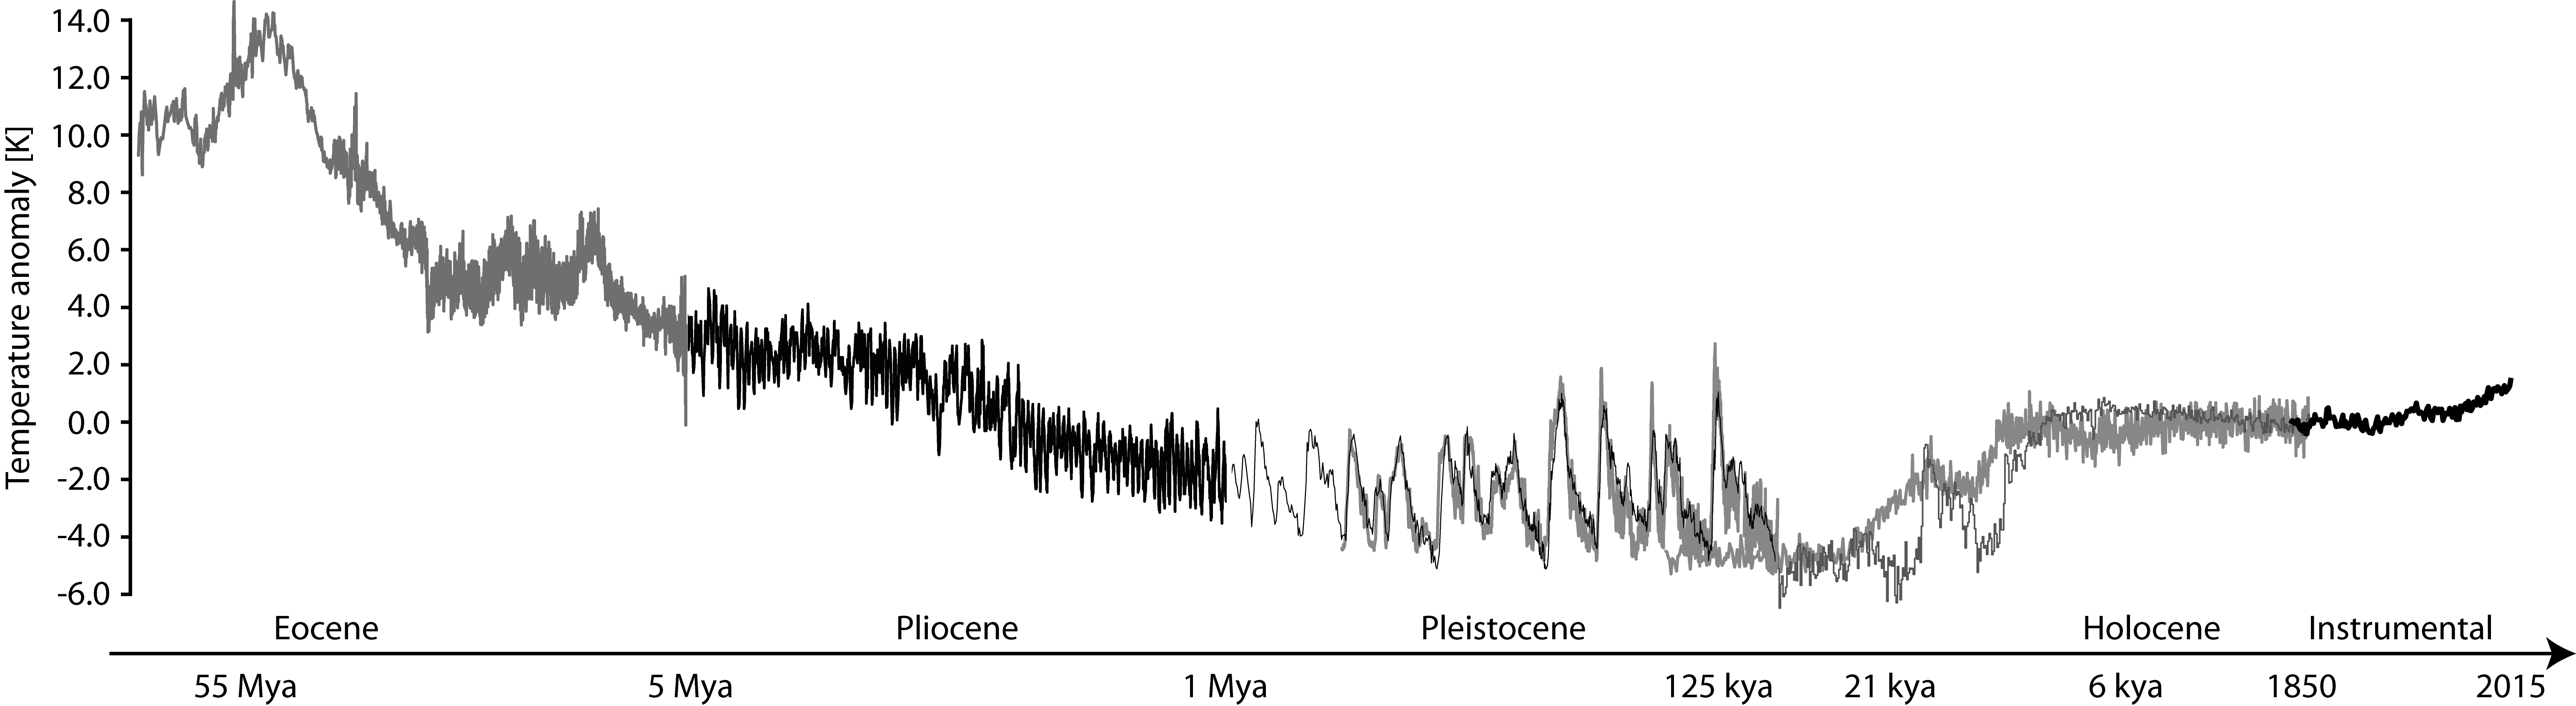
\includegraphics[width=15 cm]{../external_figures/Paleo_temperature_timeseries}
\end{center}
\caption{ Concatenation of various proxies of temperature from the past for illustration purposes. Note the logarithmic time-axis. Modified from the original by Glen Fergus. } 
\label{fig:Paleo_temperature_timeseries}
\end{figure}


\section{Climate stability}
In one perspective the Earth's climate has varied in rich ways in the past, in another perspective it has been remarkably stable (Figure \ref{fig:Paleo_temperature_timeseries}). The past 6.000 years we have had nearly steady temperatures, a period called the Holocene. These relatively mild conditions, wherein modern human civilization developed, have been rare in the past 1.000.000 years wherein the climate has cycled between longer colder glacial interrupted by short interglacials. Before that the Earth was warmer than it is today. For instance during Pliocene CO$_2$ concentrations were close to what they are today, about 400 ppm, and temperatures higher by 2-3 K. Much earlier, during the Eocene temperatures were much warmer, maybe by 10-15 K. These differences on the one hand translated into substantially different conditions for life to unfold on the planet. On the other hand, from a physical point of view the Eocene was merely 5 percent warmer than today, as measured on an absolute temperature scale. 
On this background it makes intuitive sense to think that Earth's climate is stable to small perturbations in the context of it's known history: The system did not venture to completely different states and it did spend enough time to equilibrate at almost any temperature within the range visited since dinosaurs ruled the Earth 65 million years ago (Figure \ref{fig:Paleo_temperature_timeseries}); we shall return to estimating the time-scales for equilibrating in the next chapter. 

\begin{figure}
\begin{center}
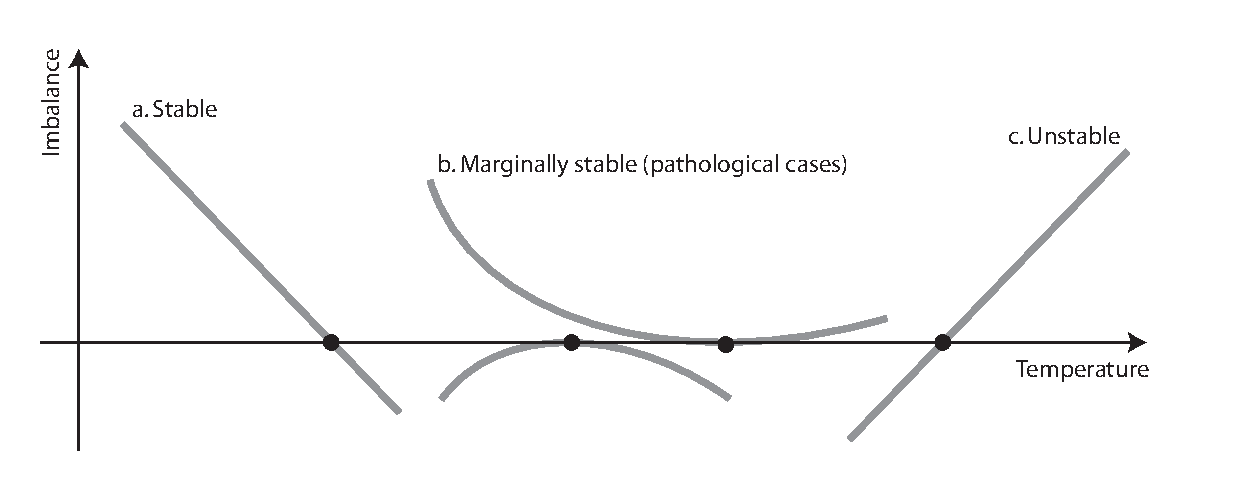
\includegraphics[width=17 cm]{../illustrations/Feedback_stability_cases.pdf}
\end{center}
\caption{ Illustration of stability cases near stationary states as marked by the black dots whereat imbalance is zero. I consider all the light gray cases where $d N/ d T = 0$ at the fix-point as limiting cases. } 
\label{fig:feedback_stability_cases}
\end{figure}

For a state to be stable it must not only have zero imbalance ($N=0$) but it must also be stable to small perturbations. The latter requires that there must be some restoring force such that if the system finds itself a bit away from stationarity, then that force will act to move the system back towards the fix-point. We can think of these perturbations as arising due to internal variability, due to weather phenomena or climate variability, or due to external forcing such as fluctuations in the solar constant or changes in atmospheric composition for reasons we consider external to the system, e.g. anthropogenic carbon dioxide emissions. For a complex system such as the Earth's climate this may be difficult to visualize as there is a practically near-infinite number of state-variables. But for many purposes we think of the climate system as having a single state-variable, the global mean surface temperature as we did it in the previous chapter, and in this case we can visualize the problem more easily (Figure \ref{fig:feedback_stability_cases}). We can think of all the other state variables as being functions of the global mean temperature. Suppose $T_o$ is a fixed-point at which the imbalance is zero and that in {\em some region} above and below $T_o$ the imbalance, $N$, is a continuous and differentiable function of $T$. Then for cases wherein $dN/dT \ne 0$ the fix-points are either stable if $dN/dT < 0$ and unstable if $dN/dT > 0$ where the derivative is calculated at $T_o$. These two possibilities are displayed as black lines in cases a and c in Figure \ref{fig:feedback_stability_cases}. We shall refer to $dN/dT$ as the feedback parameter ($\lambda$), and the above summarizes that for cases whereat $N(T_o) = 0$ the stability is determined as follows:
\begin{eqnarray}
\lambda(T_o) < 0&:& T_o \textrm{ is a stable fix-point} \nonumber \\� 
\lambda(T_o) > 0&:& T_o \textrm{ is an unstable fix-point} \nonumber
\end{eqnarray}
which is the take-home message of this section.

We talked above about stability in {\em some region} around a fix-point, but what does that mean? How large does the region have to be? It depends on how large the perturbations considered to be relevant are, if there is a faint risk of approaching another fix-point. If a stable and an unstable fix-point exists in immediate vicinity, such as shown by the dashed line in Figure \ref{fig:feedback_stability_cases}, then the stable solution is only stable to small perturbations. If it is pushed hard to temperatures above those of the unstable fix-point, then it will not return to the stable fix-point, but instead continue to warm because there $N>0$. Eventually, then system may then encounter another stable fix-point and settle in at warmer temperatures. 

In the rare limiting cases wherein both $N=0$ and $dN/dT = 0$ at the fix point things get a bit more complicated. In this case it makes sense to evaluate $N$ on either side of the fix point. If $N>0$ at somewhat colder $T$ and $N<0$ at slightly warmer $T$ then the system is stable to small perturbations, as illustrated for the gray case a in Figure \ref{fig:feedback_stability_cases}. The same argument can be used for the limiting unstable case, c. In the marginally stable cases (b) wherein $N$ has the same sign on either side of the fix-point the system is stable to perturbations in one direction and unstable to perturbations in the other direction. Think of yourself as standing on a small plateau on the side of a slippery cliff. If you try to climb up the mountain you will slide back towards the plateau (stable), but if you move a bit in the other direction you fall off the cliff and never get back to your starting point (unstable). Marginally stable fix-points occur when a system undergoes so-called bifurcations, a topic we shall return to in a later chapter.

Now let us be more concrete in applying the stability criterion we derived above. We will start with a version of the energy balance equation that you developed in an exercise of the previous chapter. In this case the greenhouse effect is represented by an effective emissivity, $\epsilon$, which is less than or equal to unity:
\begin{equation}
N = \frac{S_o}{4}(1-\alpha) - \epsilon \sigma T_s^4,
\end{equation}
from which we can estimate the feedback parameter by taking the derivative yielding:
\begin{equation}
\lambda = -\frac{S_o}{4}\frac{d\alpha}{dT_s} - \sigma T_s^4 \frac{d\epsilon}{dT_s} - 4 \epsilon \sigma T_s^3,
\label{eq:lambda_general}
\end{equation}
in the general case where $\epsilon$ and $\alpha$ are dependent on temperature. We can think of the first term as shortwave feedback which arises due to changes in planetary albedo. The origin of such feedbacks could be changes in surface albedo, e.g. through the melting of bright snow and ice, or through changes in the cloudiness. The two other terms are infrared or longwave feedbacks. The middle term encapsulates changes in the Earth's emissivity with temperature, as we shall see e.g. due to increasing water vapor and rising upper-level clouds with warming. The last term is what is often referred to as the Planck feedback.

If we consider a system with constant $\epsilon$ and $\alpha$ then the only term remaining is the Planck feedback for which we have:
\begin{equation}
\lambda_P = - 4 \epsilon \sigma T_s^3 < 0 
\end{equation}
for all $T_s$ implying that this system is unconditionally stable. If we insert numbers typical for the Earth we obtain obtain $\lambda_p \approx$ -3.25 Wm$^{-2}$K$^{-1}$ which is surprisingly close to the value obtained from complex climate models. The second term on the right hand side of equation \ref{eq:lambda_general}, which is broadly to be thought of as water vapor feedback, is found in climate models to be about +1 Wm$^{-2}$K$^{-1}$ (we shall refine this below), and so is not sufficient to cause instability in current climates. In warmer climates the positive water vapor feedback is thought to increase faster than the negative Planck feedback and so could aid in destabilising the system. It is left as an exercise to estimate the criterion for instability when considering planetary albedo feedback.

\section{Feedback mechanisms}
Above we calculated the feedback parameter for the general case (Eq. \ref{eq:lambda_general}) and identified three terms, one related to how planetary albedo changes with temperature one related to how the effective emissivity changes and one which is directly related to the Planck feedback. Now, if we want to go about understanding and quantifying the feedback it is more convenient to make another division. For instance the planetary albedo is controlled by changes in surface albedo, cloudiness and water vapor, as well as some other factors such as aerosol particles and ozone that we shall ignore here as feedbacks. 
As a first step let us divide $\lambda$ into contributions due to changes in temperature, water vapor, surface albedo and clouds:
\begin{equation}
\lambda =  \lambda_T + \lambda_W + \lambda_A + \lambda_C + ...
\end{equation}
where there are a number of additional terms due to interactions between e.g. clouds and water vapor changes as well as other factors that we have ignored (aerosols, ozone etc.). As long as we consider relatively small perturbations  then the interactions between feedbacks are of secondary importance. For large perturbations, however, it is easy to appreciate that this will no longer be the case. For instance cloudiness tends to increase in a warming climate, and so a decreasing surface albedo will have less of an impact on the energy imbalance than in a colder case. Or if the vertical temperature structure is substantially altered due to a rising tropopause, then the impacts of clouds and water vapor changes on the greenhouse effect may be different.

It turns out to be meaningful to divide the temperature feedback parameter into two contributions. 
\begin{equation}
\lambda_T \approx \lambda_P + \lambda_{LR}
\end{equation}


Complex climate models agree broadly on the importance of these feedback mechanisms, although the strengths of feedback parameters are model dependent. Table \ref{table:feedbacks} shows a dozen examples from some of the models that participated in the latest Coupled Model Intercomparison Project (CMIP5). In particular the cloud feedback parameter varies substantially among models.

\begin{table}
  \caption{ Overview of feedback parameter strength in some climate models as diagnosed using the radiative kernel method. This is a subset of the analysis from Vial et al. (2013). }
  \vspace{0.5 cm}
  \centering
  \begin{tabular}{l|rrrrrr} 
    Model                 & $\lambda_P$ & $\lambda_{LR}$ & $\lambda_W$ & $\lambda_{W+LR}$ & $\lambda_A$ & $\lambda_C$ \\
    \hline
    IPSL-CM5A-LR  & -3.29 & -0.97 & 1.86 & 0.89 & 0.18 & 1.18 \\
    NorESM1-M       & -3.19 & -0.47 & 1.54 & 1.07 & 0.30 & 0.14 \\
    MPI-ESM-LR      & -3.27 & -0.88 & 1.76 & 0.89 & 0.29 & 0.45 \\
    INMCM4             & -3.24 & -0.67 & 1.62 & 0.95 & 0.33 & -0.05 \\
    HadGEM2          & -3.18 & -0.55 & 1.49 & 0.94 & 0.29 & 0.39 \\
    CanESM2          & -3.23 & -0.64 & 1.67 & 1.03 & 0.32 & 0.52 \\
    MIROC5             & -3.22 & -0.66 & 1.68 & 1.02 & 0.36 & 0.04 \\
    CCSM4              & -3.18 & -0.44 & 1.48 & 1.05 & 0.40 & -0.42 \\
    BNU-ESM          & -3.15 & -0.22 & 1.39 & 1.17 & 0.48 & 0.09 \\
    FGOALS-s2       & -3.20 & -0.53 & 1.73 & 1.20 & 0.37 & -0.10 \\
    MRI-CGCM3      & -3.22 & -0.61 & 1.53 & 0.92 & 0.37 & 0.21 \\
    \hline
    Ensemble mean      & -3.22 & -0.60 & 1.61 & 1.01 & 0.34 & 0.22 \\
    Standard deviation  & 0.04 & 0.21 & 0.14 & 0.11 & 0.08 & 0.42 \\
  \end{tabular}
  \label{table:feedbacks}
\end{table}

\subsection{Surface albedo feedback}


\subsection{Water vapor feedback}

\begin{eqnarray}
\frac{de_s}{dT} &=& \frac{L_v e_s}{R_v T^2}, \nonumber \\
\frac{d\ln e_s}{dT} &=& \frac{L_v}{R_v T^2}
\label{eq:clausius_clapeyron}
\end{eqnarray}


\subsection{Cloud feedbacks}






\section{Equilibrium climate sensitivity (ECS)}


\begin{figure}
\begin{center}
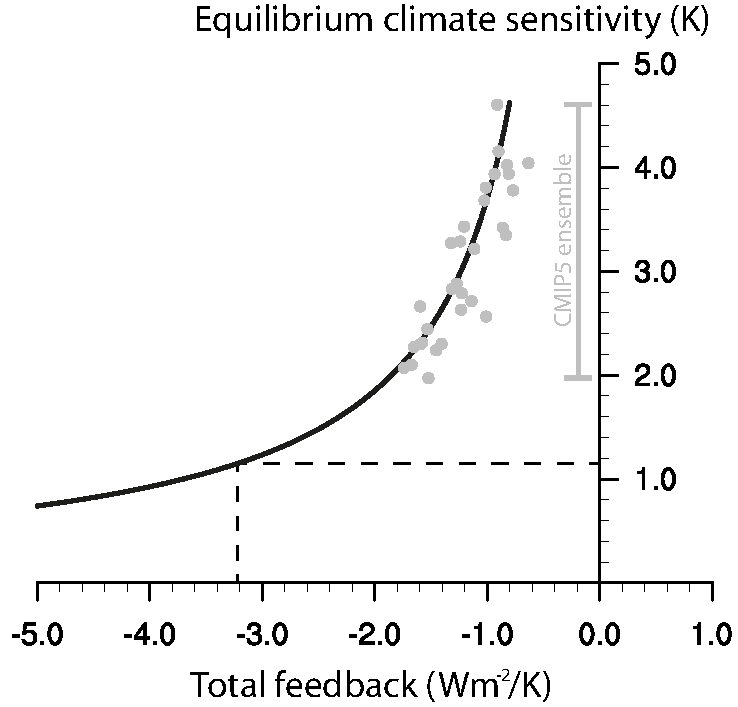
\includegraphics[width=8 cm]{../external_figures/Feedback_vs_ECS.pdf}
\end{center}
\caption{ Relationship between feedback and equilibrium climate sensitivity to one doubling of CO$_2$, ie. a forcing of 3.7 Wm$^{-2}$. Gray dots show individual CMIP5 climate models, and the dashed line indicates the case with only Planck feedback ($\lambda=\lambda_P$). } 
\label{fig:feedback_vs_ECS}
\end{figure}




\vspace{1 cm}
{\setlength{\parindent}{0cm}
\hrule
\begin{exercise}
Estimate the limit of instability for planetary albedo feedbacks using equation \ref{eq:lambda_general}. First assume $\epsilon$ is a constant. Put in numbers relevant for Earth to estimate how fast planetary albedo would have to decrease to alone cause instability.  
\end{exercise}

\begin{exercise}
Use the online MODTRAN radiative transfer model to estimate water vapor feedback. Do so by changing the 'Water Vapor Scale' from, say, 1.00 to 1.07, corresponding to a 7 percent increase of specific humidity which is roughly what occurs for a 1 K warming at typical tropospheric temperatures. Another way to do this is to use the 'Ground T offset', which actually increases the temperature of the whole column, then compare the cases with constant vapor pressure and relative humidity. It is convenient to use the 'Save this run to background' button.

How does the water vapor feedback depend on locality? How does your estimate compare with that of complex climate models?
\end{exercise}



}


%---------------------------------------------------------------------
\chapter{Temporal evolution}
\section{Heat capacities and time-scales}
\section{Mixed-layer ocean}
%\subsection{Step-response solution}
\section{Two-layer model}
\section{Zero-layer model}
\section{Sea-level rise}

%---------------------------------------------------------------------
\chapter{Forcing and adjustments}

%---------------------------------------------------------------------
\chapter{Historical warming}

%---------------------------------------------------------------------
\chapter{Time- and state-dependent feedback}
\section{Snow-ball Earth instability}
\section{Runaway feedback}
\section{Ocean heat uptake efficacy}

%---------------------------------------------------------------------
\chapter{The water cycle}


%---------------------------------------------------------------------
\chapter{Projects}


\section{Attribution of historical warming}


\section{MODTRAN exercise}


\section{Modeling natural variability}


\section{Treating volcanoes in historical simulations}


\section{Estimate Earth's climate sensitivity from historical warming}


\section{Fit two-layer model to GCM}





%\begin{figure}
%\begin{center}
%\includegraphics[width=8 cm]{../Commitment_estimates_plots/Figure_1_ECS_TCR}
%\end{center}
%\caption{ \small Probabilities of the transient climate response TCR and the equilibrium climate sensitivity ECS based on observed warming, estimates of historical radiative forcing and observations of present-day energy imbalance (a). The lower panel (b) shows the ratio of these quantities, which is roughly equivalent to the proportion of long-term warming realized on centennial time scales. Displayed numbers are the median and 5-95 percentiles of each distribution. } 
%\label{fig:ecs_tcr}
%\end{figure}

%--------------------------------------------------------%
\newpage
\bibliographystyle{naturemag}
\bibliography{bibliography}
%--------------------------------------------------------%

\vspace{5 mm}
\noindent
{\bf Acknowledgements} 



\newpage

\begin{table}
  \caption{Input for the observations-based analysis. Changes are between the period 2005-2015 minus 1859-1882. Uncertainties are standard deviations of the assumed gaussian distributions. The lower part of the table specifies the individual contributions to the total forcing change, whereas the total aerosol forcing ($F_\textrm{aero}$) is relative to 1750. }
  \vspace{0.5 cm}
  \centering
  \begin{tabular}{lrlr}
    \hline
    Quantity & Value &  & Source\\
    \hline
    Temperature change ($\Delta T$)     & 0.77&$\pm$ 0.08 K                  & HadCRUT4\citep{Morice:2012dw} \\
    Total forcing change ($\Delta F$)      & 2.16&$\pm$ 0.59 Wm$^{-2}$   & IPCC\citep{IPCC:2013is} \\    
    Planetary imbalance, 2005-2015 ($Q$)            & 0.71&$\pm$ 0.06 Wm$^{-2}$   & Johnson et al.\citep{Johnson:2016do} \\
    Planetary imbalance, 1859-1882                      & 0.15&$\pm$ 0.075 Wm$^{-2}$ & Lewis and Curry\citep{Lewis:2014jt} \\    
    \hline
    Greenhouse gas forcing change   & 2.53&$\pm$ 0.18 Wm$^{-2}$   & IPCC\citep{IPCC:2013is} \\    
    Aerosol forcing change                  &-0.69&$\pm$ 0.55 Wm$^{-2}$   & IPCC\citep{IPCC:2013is} \\    
    Black carbon on snow change      & 0.02&$\pm$ 0.02 Wm$^{-2}$   & IPCC\citep{IPCC:2013is} \\     
    Stratospheric water vapor change& 0.06&$\pm$ 0.03 Wm$^{-2}$   & IPCC\citep{IPCC:2013is} \\        
    Land use change                          &-0.10&$\pm$ 0.06 Wm$^{-2}$   & IPCC\citep{IPCC:2013is} \\        
    Ozone change                              & 0.29&$\pm$ 0.12 Wm$^{-2}$   & IPCC\citep{IPCC:2013is} \\        
    Contrails                                        & 0.05& Wm$^{-2}$                     & IPCC\citep{IPCC:2013is} \\        
    Natural forcing change                  & -0.005 &  Wm$^{-2}$                & IPCC\citep{IPCC:2013is} \\         
    \hline
    Forcing for doubled CO$_2$ ($F_{2\times}$)           & 3.71&$\pm$ 0.26 Wm$^{-2}$   & \\        
    Total aerosol forcing, 2005-2015 ($F_\textrm{aero}$)  &-0.90&$\pm$ 0.55 Wm$^{-2}$   & \\      
    \hline
  \end{tabular}

  \label{table:input}
\end{table}

\begin{table}
  \caption{ Input for calculation of short-lived climate forcers associated with fossil fuel burning. Uncertainties are standard deviations calculated from the referenced 5-95 percentiles. }
  \vspace{0.5 cm}
  \centering
  \begin{tabular}{lrlr}
    \hline
    Quantity & Value &  & Source\\
    \hline
    Methane (CH$_4$)              & 0.970 &$\pm$ 0.10 Wm$^{-2}$                  & IPCC\citep{Myhre:2013ui} \\
    Nitrogen oxides (NO$_x$)     & -0.151 &$\pm$ 0.11 Wm$^{-2}$                  & IPCC\citep{Myhre:2013ui} \\
    Carbon monoxide (CO)       & 0.234 &$\pm$ 0.03 Wm$^{-2}$                  & IPCC\citep{Myhre:2013ui} \\
    Fossil fuel fraction of CH$_4$ emissions ($f_{ff}$) & 0.29 &$\pm$ 0.02   & IPCC\citep{Ciais:2013ui} \\
    \hline
    Weighted sum (F$_\textrm{slcf}$)      & 0.36   &$\pm$ 0.12 Wm$^{-2}$                  & \\
    \hline
  \end{tabular}

  \label{table:slcfs}
\end{table}



\end{document}

